% Options for packages loaded elsewhere
\PassOptionsToPackage{unicode}{hyperref}
\PassOptionsToPackage{hyphens}{url}
%
\documentclass[
]{book}
\usepackage{amsmath,amssymb}
\usepackage{lmodern}
\usepackage{ifxetex,ifluatex}
\ifnum 0\ifxetex 1\fi\ifluatex 1\fi=0 % if pdftex
  \usepackage[T1]{fontenc}
  \usepackage[utf8]{inputenc}
  \usepackage{textcomp} % provide euro and other symbols
\else % if luatex or xetex
  \usepackage{unicode-math}
  \defaultfontfeatures{Scale=MatchLowercase}
  \defaultfontfeatures[\rmfamily]{Ligatures=TeX,Scale=1}
\fi
% Use upquote if available, for straight quotes in verbatim environments
\IfFileExists{upquote.sty}{\usepackage{upquote}}{}
\IfFileExists{microtype.sty}{% use microtype if available
  \usepackage[]{microtype}
  \UseMicrotypeSet[protrusion]{basicmath} % disable protrusion for tt fonts
}{}
\makeatletter
\@ifundefined{KOMAClassName}{% if non-KOMA class
  \IfFileExists{parskip.sty}{%
    \usepackage{parskip}
  }{% else
    \setlength{\parindent}{0pt}
    \setlength{\parskip}{6pt plus 2pt minus 1pt}}
}{% if KOMA class
  \KOMAoptions{parskip=half}}
\makeatother
\usepackage{xcolor}
\IfFileExists{xurl.sty}{\usepackage{xurl}}{} % add URL line breaks if available
\IfFileExists{bookmark.sty}{\usepackage{bookmark}}{\usepackage{hyperref}}
\hypersetup{
  pdftitle={R Guide for TMLE in Medical Research},
  hidelinks,
  pdfcreator={LaTeX via pandoc}}
\urlstyle{same} % disable monospaced font for URLs
\usepackage{color}
\usepackage{fancyvrb}
\newcommand{\VerbBar}{|}
\newcommand{\VERB}{\Verb[commandchars=\\\{\}]}
\DefineVerbatimEnvironment{Highlighting}{Verbatim}{commandchars=\\\{\}}
% Add ',fontsize=\small' for more characters per line
\usepackage{framed}
\definecolor{shadecolor}{RGB}{248,248,248}
\newenvironment{Shaded}{\begin{snugshade}}{\end{snugshade}}
\newcommand{\AlertTok}[1]{\textcolor[rgb]{0.94,0.16,0.16}{#1}}
\newcommand{\AnnotationTok}[1]{\textcolor[rgb]{0.56,0.35,0.01}{\textbf{\textit{#1}}}}
\newcommand{\AttributeTok}[1]{\textcolor[rgb]{0.77,0.63,0.00}{#1}}
\newcommand{\BaseNTok}[1]{\textcolor[rgb]{0.00,0.00,0.81}{#1}}
\newcommand{\BuiltInTok}[1]{#1}
\newcommand{\CharTok}[1]{\textcolor[rgb]{0.31,0.60,0.02}{#1}}
\newcommand{\CommentTok}[1]{\textcolor[rgb]{0.56,0.35,0.01}{\textit{#1}}}
\newcommand{\CommentVarTok}[1]{\textcolor[rgb]{0.56,0.35,0.01}{\textbf{\textit{#1}}}}
\newcommand{\ConstantTok}[1]{\textcolor[rgb]{0.00,0.00,0.00}{#1}}
\newcommand{\ControlFlowTok}[1]{\textcolor[rgb]{0.13,0.29,0.53}{\textbf{#1}}}
\newcommand{\DataTypeTok}[1]{\textcolor[rgb]{0.13,0.29,0.53}{#1}}
\newcommand{\DecValTok}[1]{\textcolor[rgb]{0.00,0.00,0.81}{#1}}
\newcommand{\DocumentationTok}[1]{\textcolor[rgb]{0.56,0.35,0.01}{\textbf{\textit{#1}}}}
\newcommand{\ErrorTok}[1]{\textcolor[rgb]{0.64,0.00,0.00}{\textbf{#1}}}
\newcommand{\ExtensionTok}[1]{#1}
\newcommand{\FloatTok}[1]{\textcolor[rgb]{0.00,0.00,0.81}{#1}}
\newcommand{\FunctionTok}[1]{\textcolor[rgb]{0.00,0.00,0.00}{#1}}
\newcommand{\ImportTok}[1]{#1}
\newcommand{\InformationTok}[1]{\textcolor[rgb]{0.56,0.35,0.01}{\textbf{\textit{#1}}}}
\newcommand{\KeywordTok}[1]{\textcolor[rgb]{0.13,0.29,0.53}{\textbf{#1}}}
\newcommand{\NormalTok}[1]{#1}
\newcommand{\OperatorTok}[1]{\textcolor[rgb]{0.81,0.36,0.00}{\textbf{#1}}}
\newcommand{\OtherTok}[1]{\textcolor[rgb]{0.56,0.35,0.01}{#1}}
\newcommand{\PreprocessorTok}[1]{\textcolor[rgb]{0.56,0.35,0.01}{\textit{#1}}}
\newcommand{\RegionMarkerTok}[1]{#1}
\newcommand{\SpecialCharTok}[1]{\textcolor[rgb]{0.00,0.00,0.00}{#1}}
\newcommand{\SpecialStringTok}[1]{\textcolor[rgb]{0.31,0.60,0.02}{#1}}
\newcommand{\StringTok}[1]{\textcolor[rgb]{0.31,0.60,0.02}{#1}}
\newcommand{\VariableTok}[1]{\textcolor[rgb]{0.00,0.00,0.00}{#1}}
\newcommand{\VerbatimStringTok}[1]{\textcolor[rgb]{0.31,0.60,0.02}{#1}}
\newcommand{\WarningTok}[1]{\textcolor[rgb]{0.56,0.35,0.01}{\textbf{\textit{#1}}}}
\usepackage{longtable,booktabs,array}
\usepackage{calc} % for calculating minipage widths
% Correct order of tables after \paragraph or \subparagraph
\usepackage{etoolbox}
\makeatletter
\patchcmd\longtable{\par}{\if@noskipsec\mbox{}\fi\par}{}{}
\makeatother
% Allow footnotes in longtable head/foot
\IfFileExists{footnotehyper.sty}{\usepackage{footnotehyper}}{\usepackage{footnote}}
\makesavenoteenv{longtable}
\usepackage{graphicx}
\makeatletter
\def\maxwidth{\ifdim\Gin@nat@width>\linewidth\linewidth\else\Gin@nat@width\fi}
\def\maxheight{\ifdim\Gin@nat@height>\textheight\textheight\else\Gin@nat@height\fi}
\makeatother
% Scale images if necessary, so that they will not overflow the page
% margins by default, and it is still possible to overwrite the defaults
% using explicit options in \includegraphics[width, height, ...]{}
\setkeys{Gin}{width=\maxwidth,height=\maxheight,keepaspectratio}
% Set default figure placement to htbp
\makeatletter
\def\fps@figure{htbp}
\makeatother
\setlength{\emergencystretch}{3em} % prevent overfull lines
\providecommand{\tightlist}{%
  \setlength{\itemsep}{0pt}\setlength{\parskip}{0pt}}
\setcounter{secnumdepth}{5}
<script type="text/javascript">

// toggle visibility of R source blocks in R Markdown output
function toggle_R() {
  var x = document.getElementsByClassName('r');
  if (x.length == 0) return;
  function toggle_vis(o) {
    var d = o.style.display;
    o.style.display = (d == 'block' || d == '') ? 'none':'block';
  }

  for (i = 0; i < x.length; i++) {
    var y = x[i];
    if (y.tagName.toLowerCase() === 'pre') toggle_vis(y);
  }

    var elem = document.getElementById("myButton1");
    if (elem.value === "Hide Global") elem.value = "Show Global";
    else elem.value = "Hide Global";
}

document.write('<input onclick="toggle_R();" type="button" value="Hide Global" id="myButton1" style="position: absolute; top: 10%; right: 2%; z-index: 200"></input>')

</script>
\usepackage{booktabs}
\usepackage{longtable}
\usepackage{array}
\usepackage{multirow}
\usepackage{wrapfig}
\usepackage{float}
\usepackage{colortbl}
\usepackage{pdflscape}
\usepackage{tabu}
\usepackage{threeparttable}
\usepackage{threeparttablex}
\usepackage[normalem]{ulem}
\usepackage{makecell}
\usepackage{xcolor}
\ifluatex
  \usepackage{selnolig}  % disable illegal ligatures
\fi
\usepackage[]{natbib}
\bibliographystyle{apalike}
\newlength{\cslhangindent}
\setlength{\cslhangindent}{1.5em}
\newlength{\csllabelwidth}
\setlength{\csllabelwidth}{3em}
\newenvironment{CSLReferences}[2] % #1 hanging-ident, #2 entry spacing
 {% don't indent paragraphs
  \setlength{\parindent}{0pt}
  % turn on hanging indent if param 1 is 1
  \ifodd #1 \everypar{\setlength{\hangindent}{\cslhangindent}}\ignorespaces\fi
  % set entry spacing
  \ifnum #2 > 0
  \setlength{\parskip}{#2\baselineskip}
  \fi
 }%
 {}
\usepackage{calc}
\newcommand{\CSLBlock}[1]{#1\hfill\break}
\newcommand{\CSLLeftMargin}[1]{\parbox[t]{\csllabelwidth}{#1}}
\newcommand{\CSLRightInline}[1]{\parbox[t]{\linewidth - \csllabelwidth}{#1}\break}
\newcommand{\CSLIndent}[1]{\hspace{\cslhangindent}#1}

\title{R Guide for TMLE in Medical Research}
\author{}
\date{\vspace{-2.5em}2021-08-18}

\begin{document}
\maketitle

{
\setcounter{tocdepth}{1}
\tableofcontents
}
\hypertarget{preface}{%
\chapter*{Preface}\label{preface}}
\addcontentsline{toc}{chapter}{Preface}

\hypertarget{background}{%
\section*{Background}\label{background}}
\addcontentsline{toc}{section}{Background}

In comparative effectiveness studies, researchers typically use propensity score methods. However, propensity score methods have known limitations in real-world scenarios, when the true data generating mechanism is unknown. Targeted maximum likelihood estimation (TMLE) is an alternative estimation method with a number of desirable statistical properties. It is a doubly robust method, making use of both the outcome model and propensity score model to generate an unbiased estimate as long as at least one of the models is correctly specified. TMLE also enables the integration of machine learning approaches. Despite the fact that this method has been shown to perform better than propensity score methods in a variety of scenarios, it is not widely used in medical research as the technical details of this approach are generally not well understood.

change

\hypertarget{goal}{%
\section*{Goal}\label{goal}}
\addcontentsline{toc}{section}{Goal}

In this workshop we will present an introductory tutorial explaining an overview of TMLE using one real epidemiological data, the steps to use the method in R, and a demonstration of relevant R packages.~

\hypertarget{philosophy}{%
\section*{Philosophy}\label{philosophy}}
\addcontentsline{toc}{section}{Philosophy}

Code-first philosophy is adopted for this workshop; demonstrating the analyses through one real data analysis problem used in the literature. This workshop is not theory-focused, nor utilizes simulated data to explain the ideas.

\hypertarget{pre-requisites}{%
\section*{Pre-requisites}\label{pre-requisites}}
\addcontentsline{toc}{section}{Pre-requisites}

Basic understanding of \emph{R} language is required. A general understanding of \emph{multiple regression} is expected. Familiarity with \emph{machine learning} and \emph{epidemiological} core concepts would be helpful, but not required. Deep understanding of \emph{causal inference} or \emph{advanced statistical inference} knowledge is not expected.

\hypertarget{version-history}{%
\section*{Version history}\label{version-history}}
\addcontentsline{toc}{section}{Version history}

The workshop was first developed for \href{https://r-medicine.org/schedule/}{R/Medicine
Virtual Conference} 2021, August 24th; title: `An Introductory R Guide for Targeted Maximum Likelihood Estimation in Medical Research'.

\hypertarget{contributor-list}{%
\section*{Contributor list}\label{contributor-list}}
\addcontentsline{toc}{section}{Contributor list}

\begin{longtable}[]{@{}ll@{}}
\toprule
& \\
\midrule
\endhead
\href{https://www.linkedin.com/in/hanna-f-940813b9/}{Hanna Frank} (SPPH, UBC) & \href{https://ehsank.com/}{Ehsan Karim} (SPPH, UBC) \\
\bottomrule
\end{longtable}

\hypertarget{license}{%
\section*{License}\label{license}}
\addcontentsline{toc}{section}{License}


\includegraphics[width=0.25\linewidth]{images/by-nc-sa}

The online version of this book is licensed under the \href{https://creativecommons.org/licenses/by-nc-sa/4.0/}{Creative Commons Attribution-NonCommercial-ShareAlike 4.0} International License. You may share, adapt the content and may distribute your contributions under the same license (CC BY-NC-SA 4.0), but you have to give appropriate credit, and cannot use material for the commercial purposes.

\hypertarget{rhc-data-description}{%
\chapter{RHC data description}\label{rhc-data-description}}

There is a widespread belief among cardiologists that the right heart catheterization (RHC hereafter; a monitoring device for measurement of cardiac function) is helpful in managing critically ill patients in the intensive care unit. \citet{connors1996effectiveness} examined the association of

\begin{itemize}
\tightlist
\item
  \emph{RHC use} during the first 24 hours of care in the intensive care unit and
\item
  a number of health-outcomes such as \emph{length of stay} (hospital).
\end{itemize}

\hypertarget{data-download}{%
\section{Data download}\label{data-download}}

Data is freely available from \href{https://hbiostat.org/data/}{Vanderbilt Biostatistics}.

\begin{Shaded}
\begin{Highlighting}[]
\CommentTok{\# load the dataset}
\NormalTok{ObsData }\OtherTok{\textless{}{-}} \FunctionTok{read.csv}\NormalTok{(}\StringTok{"https://hbiostat.org/data/repo/rhc.csv"}\NormalTok{, }\AttributeTok{header =} \ConstantTok{TRUE}\NormalTok{)}
\FunctionTok{saveRDS}\NormalTok{(ObsData, }\AttributeTok{file =} \StringTok{"data/rhc.RDS"}\NormalTok{)}
\end{Highlighting}
\end{Shaded}

\hypertarget{analytic-data}{%
\section{Analytic data}\label{analytic-data}}

\begin{Shaded}
\begin{Highlighting}[]
\CommentTok{\# add column for outcome Y: length of stay }
\CommentTok{\# Y = date of discharge {-} study admission date}
\CommentTok{\# Y = date of death {-} study admission date if date of discharge not available}
\NormalTok{ObsData}\SpecialCharTok{$}\NormalTok{Y }\OtherTok{\textless{}{-}}\NormalTok{ ObsData}\SpecialCharTok{$}\NormalTok{dschdte }\SpecialCharTok{{-}}\NormalTok{ ObsData}\SpecialCharTok{$}\NormalTok{sadmdte}
\NormalTok{ObsData}\SpecialCharTok{$}\NormalTok{Y[}\FunctionTok{is.na}\NormalTok{(ObsData}\SpecialCharTok{$}\NormalTok{Y)] }\OtherTok{\textless{}{-}}\NormalTok{ ObsData}\SpecialCharTok{$}\NormalTok{dthdte[}\FunctionTok{is.na}\NormalTok{(ObsData}\SpecialCharTok{$}\NormalTok{Y)] }\SpecialCharTok{{-}} 
\NormalTok{  ObsData}\SpecialCharTok{$}\NormalTok{sadmdte[}\FunctionTok{is.na}\NormalTok{(ObsData}\SpecialCharTok{$}\NormalTok{Y)]}
\CommentTok{\# remove outcomes we are not examining in this example}
\NormalTok{ObsData }\OtherTok{\textless{}{-}}\NormalTok{ dplyr}\SpecialCharTok{::}\FunctionTok{select}\NormalTok{(ObsData, }
                         \SpecialCharTok{!}\FunctionTok{c}\NormalTok{(dthdte, lstctdte, dschdte, death, t3d30, dth30, surv2md1))}
\CommentTok{\# remove unnecessary and problematic variables }
\NormalTok{ObsData }\OtherTok{\textless{}{-}}\NormalTok{ dplyr}\SpecialCharTok{::}\FunctionTok{select}\NormalTok{(ObsData, }
                         \SpecialCharTok{!}\FunctionTok{c}\NormalTok{(sadmdte, ptid, X, adld3p, urin1, cat2))}

\CommentTok{\# convert all categorical variables to factors }
\NormalTok{factors }\OtherTok{\textless{}{-}} \FunctionTok{c}\NormalTok{(}\StringTok{"cat1"}\NormalTok{, }\StringTok{"ca"}\NormalTok{, }\StringTok{"cardiohx"}\NormalTok{, }\StringTok{"chfhx"}\NormalTok{, }\StringTok{"dementhx"}\NormalTok{, }\StringTok{"psychhx"}\NormalTok{, }
             \StringTok{"chrpulhx"}\NormalTok{, }\StringTok{"renalhx"}\NormalTok{, }\StringTok{"liverhx"}\NormalTok{, }\StringTok{"gibledhx"}\NormalTok{, }\StringTok{"malighx"}\NormalTok{, }
             \StringTok{"immunhx"}\NormalTok{, }\StringTok{"transhx"}\NormalTok{, }\StringTok{"amihx"}\NormalTok{, }\StringTok{"sex"}\NormalTok{, }\StringTok{"dnr1"}\NormalTok{, }\StringTok{"ninsclas"}\NormalTok{, }
             \StringTok{"resp"}\NormalTok{, }\StringTok{"card"}\NormalTok{, }\StringTok{"neuro"}\NormalTok{, }\StringTok{"gastr"}\NormalTok{, }\StringTok{"renal"}\NormalTok{, }\StringTok{"meta"}\NormalTok{, }\StringTok{"hema"}\NormalTok{, }
             \StringTok{"seps"}\NormalTok{, }\StringTok{"trauma"}\NormalTok{, }\StringTok{"ortho"}\NormalTok{, }\StringTok{"race"}\NormalTok{, }\StringTok{"income"}\NormalTok{)}
\NormalTok{ObsData[factors] }\OtherTok{\textless{}{-}} \FunctionTok{lapply}\NormalTok{(ObsData[factors], as.factor)}
\CommentTok{\# convert our treatment A (RHC vs. No RHC) to a binary variable}
\NormalTok{ObsData}\SpecialCharTok{$}\NormalTok{A }\OtherTok{\textless{}{-}} \FunctionTok{ifelse}\NormalTok{(ObsData}\SpecialCharTok{$}\NormalTok{swang1 }\SpecialCharTok{==} \StringTok{"RHC"}\NormalTok{, }\DecValTok{1}\NormalTok{, }\DecValTok{0}\NormalTok{)}
\NormalTok{ObsData }\OtherTok{\textless{}{-}}\NormalTok{ dplyr}\SpecialCharTok{::}\FunctionTok{select}\NormalTok{(ObsData, }\SpecialCharTok{!}\NormalTok{swang1)}
\CommentTok{\# Categorize the variables to match with the original paper}
\NormalTok{ObsData}\SpecialCharTok{$}\NormalTok{age }\OtherTok{\textless{}{-}} \FunctionTok{cut}\NormalTok{(ObsData}\SpecialCharTok{$}\NormalTok{age,}\AttributeTok{breaks=}\FunctionTok{c}\NormalTok{(}\SpecialCharTok{{-}}\ConstantTok{Inf}\NormalTok{, }\DecValTok{50}\NormalTok{, }\DecValTok{60}\NormalTok{, }\DecValTok{70}\NormalTok{, }\DecValTok{80}\NormalTok{, }\ConstantTok{Inf}\NormalTok{),}\AttributeTok{right=}\ConstantTok{FALSE}\NormalTok{)}
\NormalTok{ObsData}\SpecialCharTok{$}\NormalTok{race }\OtherTok{\textless{}{-}} \FunctionTok{factor}\NormalTok{(ObsData}\SpecialCharTok{$}\NormalTok{race, }\AttributeTok{levels=}\FunctionTok{c}\NormalTok{(}\StringTok{"white"}\NormalTok{,}\StringTok{"black"}\NormalTok{,}\StringTok{"other"}\NormalTok{))}
\NormalTok{ObsData}\SpecialCharTok{$}\NormalTok{sex }\OtherTok{\textless{}{-}} \FunctionTok{as.factor}\NormalTok{(ObsData}\SpecialCharTok{$}\NormalTok{sex)}
\NormalTok{ObsData}\SpecialCharTok{$}\NormalTok{sex }\OtherTok{\textless{}{-}} \FunctionTok{relevel}\NormalTok{(ObsData}\SpecialCharTok{$}\NormalTok{sex, }\AttributeTok{ref =} \StringTok{"Male"}\NormalTok{)}
\NormalTok{ObsData}\SpecialCharTok{$}\NormalTok{cat1 }\OtherTok{\textless{}{-}} \FunctionTok{as.factor}\NormalTok{(ObsData}\SpecialCharTok{$}\NormalTok{cat1)}
\FunctionTok{levels}\NormalTok{(ObsData}\SpecialCharTok{$}\NormalTok{cat1) }\OtherTok{\textless{}{-}} \FunctionTok{c}\NormalTok{(}\StringTok{"ARF"}\NormalTok{,}\StringTok{"CHF"}\NormalTok{,}\StringTok{"Other"}\NormalTok{,}\StringTok{"Other"}\NormalTok{,}\StringTok{"Other"}\NormalTok{,}
                          \StringTok{"Other"}\NormalTok{,}\StringTok{"Other"}\NormalTok{,}\StringTok{"MOSF"}\NormalTok{,}\StringTok{"MOSF"}\NormalTok{)}
\NormalTok{ObsData}\SpecialCharTok{$}\NormalTok{ca }\OtherTok{\textless{}{-}} \FunctionTok{as.factor}\NormalTok{(ObsData}\SpecialCharTok{$}\NormalTok{ca)}
\FunctionTok{levels}\NormalTok{(ObsData}\SpecialCharTok{$}\NormalTok{ca) }\OtherTok{\textless{}{-}} \FunctionTok{c}\NormalTok{(}\StringTok{"Metastatic"}\NormalTok{,}\StringTok{"None"}\NormalTok{,}\StringTok{"Localized (Yes)"}\NormalTok{)}
\NormalTok{ObsData}\SpecialCharTok{$}\NormalTok{ca }\OtherTok{\textless{}{-}} \FunctionTok{factor}\NormalTok{(ObsData}\SpecialCharTok{$}\NormalTok{ca, }\AttributeTok{levels=}\FunctionTok{c}\NormalTok{(}\StringTok{"None"}\NormalTok{,}
                                          \StringTok{"Localized (Yes)"}\NormalTok{,}\StringTok{"Metastatic"}\NormalTok{))}
\CommentTok{\# Rename variables}
\FunctionTok{names}\NormalTok{(ObsData) }\OtherTok{\textless{}{-}} \FunctionTok{c}\NormalTok{(}\StringTok{"Disease.category"}\NormalTok{, }\StringTok{"Cancer"}\NormalTok{, }\StringTok{"Cardiovascular"}\NormalTok{, }
                    \StringTok{"Congestive.HF"}\NormalTok{, }\StringTok{"Dementia"}\NormalTok{, }\StringTok{"Psychiatric"}\NormalTok{, }\StringTok{"Pulmonary"}\NormalTok{, }
                    \StringTok{"Renal"}\NormalTok{, }\StringTok{"Hepatic"}\NormalTok{, }\StringTok{"GI.Bleed"}\NormalTok{, }\StringTok{"Tumor"}\NormalTok{, }
                    \StringTok{"Immunosupperssion"}\NormalTok{, }\StringTok{"Transfer.hx"}\NormalTok{, }\StringTok{"MI"}\NormalTok{, }\StringTok{"age"}\NormalTok{, }\StringTok{"sex"}\NormalTok{, }
                    \StringTok{"edu"}\NormalTok{, }\StringTok{"DASIndex"}\NormalTok{, }\StringTok{"APACHE.score"}\NormalTok{, }\StringTok{"Glasgow.Coma.Score"}\NormalTok{, }
                    \StringTok{"blood.pressure"}\NormalTok{, }\StringTok{"WBC"}\NormalTok{, }\StringTok{"Heart.rate"}\NormalTok{, }\StringTok{"Respiratory.rate"}\NormalTok{, }
                    \StringTok{"Temperature"}\NormalTok{, }\StringTok{"PaO2vs.FIO2"}\NormalTok{, }\StringTok{"Albumin"}\NormalTok{, }\StringTok{"Hematocrit"}\NormalTok{, }
                    \StringTok{"Bilirubin"}\NormalTok{, }\StringTok{"Creatinine"}\NormalTok{, }\StringTok{"Sodium"}\NormalTok{, }\StringTok{"Potassium"}\NormalTok{, }\StringTok{"PaCo2"}\NormalTok{, }
                    \StringTok{"PH"}\NormalTok{, }\StringTok{"Weight"}\NormalTok{, }\StringTok{"DNR.status"}\NormalTok{, }\StringTok{"Medical.insurance"}\NormalTok{, }
                    \StringTok{"Respiratory.Diag"}\NormalTok{, }\StringTok{"Cardiovascular.Diag"}\NormalTok{, }
                    \StringTok{"Neurological.Diag"}\NormalTok{, }\StringTok{"Gastrointestinal.Diag"}\NormalTok{, }\StringTok{"Renal.Diag"}\NormalTok{,}
                    \StringTok{"Metabolic.Diag"}\NormalTok{, }\StringTok{"Hematologic.Diag"}\NormalTok{, }\StringTok{"Sepsis.Diag"}\NormalTok{, }
                    \StringTok{"Trauma.Diag"}\NormalTok{, }\StringTok{"Orthopedic.Diag"}\NormalTok{, }\StringTok{"race"}\NormalTok{, }\StringTok{"income"}\NormalTok{, }
                    \StringTok{"Y"}\NormalTok{, }\StringTok{"A"}\NormalTok{)}
\FunctionTok{saveRDS}\NormalTok{(ObsData, }\AttributeTok{file =} \StringTok{"data/rhcAnalytic.RDS"}\NormalTok{)}
\end{Highlighting}
\end{Shaded}

\hypertarget{notations}{%
\section{Notations}\label{notations}}

\begin{longtable}[]{@{}
  >{\raggedright\arraybackslash}p{(\columnwidth - 2\tabcolsep) * \real{0.50}}
  >{\raggedright\arraybackslash}p{(\columnwidth - 2\tabcolsep) * \real{0.50}}@{}}
\toprule
Notations & Example in RHC study \\
\midrule
\endhead
\(A\): Exposure status & RHC \\
\(Y\): Observed outcome & length of stay \\
\(Y(A=1)\) = potential outcome when exposed & length of stay when RHC used \\
\(Y(A=0)\) = potential outcome when not exposed & length of stay when RHC not used \\
\(L\): Covariates & See below \\
\bottomrule
\end{longtable}

\hypertarget{variables}{%
\section{Variables}\label{variables}}

\begin{Shaded}
\begin{Highlighting}[]
\NormalTok{baselinevars }\OtherTok{\textless{}{-}} \FunctionTok{names}\NormalTok{(dplyr}\SpecialCharTok{::}\FunctionTok{select}\NormalTok{(ObsData, }
                         \SpecialCharTok{!}\FunctionTok{c}\NormalTok{(A,Y)))}
\NormalTok{baselinevars}
\end{Highlighting}
\end{Shaded}

\begin{verbatim}
##  [1] "Disease.category"      "Cancer"                "Cardiovascular"       
##  [4] "Congestive.HF"         "Dementia"              "Psychiatric"          
##  [7] "Pulmonary"             "Renal"                 "Hepatic"              
## [10] "GI.Bleed"              "Tumor"                 "Immunosupperssion"    
## [13] "Transfer.hx"           "MI"                    "age"                  
## [16] "sex"                   "edu"                   "DASIndex"             
## [19] "APACHE.score"          "Glasgow.Coma.Score"    "blood.pressure"       
## [22] "WBC"                   "Heart.rate"            "Respiratory.rate"     
## [25] "Temperature"           "PaO2vs.FIO2"           "Albumin"              
## [28] "Hematocrit"            "Bilirubin"             "Creatinine"           
## [31] "Sodium"                "Potassium"             "PaCo2"                
## [34] "PH"                    "Weight"                "DNR.status"           
## [37] "Medical.insurance"     "Respiratory.Diag"      "Cardiovascular.Diag"  
## [40] "Neurological.Diag"     "Gastrointestinal.Diag" "Renal.Diag"           
## [43] "Metabolic.Diag"        "Hematologic.Diag"      "Sepsis.Diag"          
## [46] "Trauma.Diag"           "Orthopedic.Diag"       "race"                 
## [49] "income"
\end{verbatim}

\hypertarget{table-1-stratified-by-rhc-exposure}{%
\section{Table 1 stratified by RHC exposure}\label{table-1-stratified-by-rhc-exposure}}

Only for some demographic and co-morbidity variables; match with Table 1 in \citet{connors1996effectiveness}.

\begin{Shaded}
\begin{Highlighting}[]
\FunctionTok{require}\NormalTok{(tableone)}
\NormalTok{tab0 }\OtherTok{\textless{}{-}} \FunctionTok{CreateTableOne}\NormalTok{(}\AttributeTok{vars =} \FunctionTok{c}\NormalTok{(}\StringTok{"age"}\NormalTok{, }\StringTok{"sex"}\NormalTok{, }\StringTok{"race"}\NormalTok{, }\StringTok{"Disease.category"}\NormalTok{, }\StringTok{"Cancer"}\NormalTok{),}
                       \AttributeTok{data =}\NormalTok{ ObsData, }
                       \AttributeTok{strata =} \StringTok{"A"}\NormalTok{, }
                       \AttributeTok{test =} \ConstantTok{FALSE}\NormalTok{)}
\FunctionTok{print}\NormalTok{(tab0, }\AttributeTok{showAllLevels =} \ConstantTok{FALSE}\NormalTok{, )}
\end{Highlighting}
\end{Shaded}

\begin{verbatim}
##                       Stratified by A
##                        0            1           
##   n                    3551         2184        
##   age (%)                                       
##      [-Inf,50)          884 (24.9)   540 (24.7) 
##      [50,60)            546 (15.4)   371 (17.0) 
##      [60,70)            812 (22.9)   577 (26.4) 
##      [70,80)            809 (22.8)   529 (24.2) 
##      [80, Inf)          500 (14.1)   167 ( 7.6) 
##   sex = Female (%)     1637 (46.1)   906 (41.5) 
##   race (%)                                      
##      white             2753 (77.5)  1707 (78.2) 
##      black              585 (16.5)   335 (15.3) 
##      other              213 ( 6.0)   142 ( 6.5) 
##   Disease.category (%)                          
##      ARF               1581 (44.5)   909 (41.6) 
##      CHF                247 ( 7.0)   209 ( 9.6) 
##      Other              955 (26.9)   208 ( 9.5) 
##      MOSF               768 (21.6)   858 (39.3) 
##   Cancer (%)                                    
##      None              2652 (74.7)  1727 (79.1) 
##      Localized (Yes)    638 (18.0)   334 (15.3) 
##      Metastatic         261 ( 7.4)   123 ( 5.6)
\end{verbatim}

Only outcome variable (Length of stay); slightly different than Table 2 in \citet{connors1996effectiveness} (means 20.5 vs.~25.7; and medians 13 vs.~17).

\begin{Shaded}
\begin{Highlighting}[]
\NormalTok{tab1 }\OtherTok{\textless{}{-}} \FunctionTok{CreateTableOne}\NormalTok{(}\AttributeTok{vars =} \FunctionTok{c}\NormalTok{(}\StringTok{"Y"}\NormalTok{),}
                       \AttributeTok{data =}\NormalTok{ ObsData, }
                       \AttributeTok{strata =} \StringTok{"A"}\NormalTok{, }
                       \AttributeTok{test =} \ConstantTok{FALSE}\NormalTok{)}
\FunctionTok{print}\NormalTok{(tab1, }\AttributeTok{showAllLevels =} \ConstantTok{FALSE}\NormalTok{, )}
\end{Highlighting}
\end{Shaded}

\begin{verbatim}
##                Stratified by A
##                 0             1            
##   n              3551          2184        
##   Y (mean (SD)) 19.53 (23.59) 24.86 (28.90)
\end{verbatim}

\begin{Shaded}
\begin{Highlighting}[]
\FunctionTok{median}\NormalTok{(ObsData}\SpecialCharTok{$}\NormalTok{Y[ObsData}\SpecialCharTok{$}\NormalTok{A}\SpecialCharTok{==}\DecValTok{0}\NormalTok{]); }\FunctionTok{median}\NormalTok{(ObsData}\SpecialCharTok{$}\NormalTok{Y[ObsData}\SpecialCharTok{$}\NormalTok{A}\SpecialCharTok{==}\DecValTok{1}\NormalTok{])}
\end{Highlighting}
\end{Shaded}

\begin{verbatim}
## [1] 12
\end{verbatim}

\begin{verbatim}
## [1] 16
\end{verbatim}

\hypertarget{basic-regression-analysis}{%
\section{Basic regression analysis}\label{basic-regression-analysis}}

\hypertarget{crude-analysis}{%
\subsection{Crude analysis}\label{crude-analysis}}

\begin{Shaded}
\begin{Highlighting}[]
\CommentTok{\# adjust the exposure variable (primary interest)}
\NormalTok{fit0 }\OtherTok{\textless{}{-}} \FunctionTok{lm}\NormalTok{(Y}\SpecialCharTok{\textasciitilde{}}\NormalTok{A, }\AttributeTok{data =}\NormalTok{ ObsData)}
\FunctionTok{require}\NormalTok{(Publish)}
\NormalTok{crude.fit }\OtherTok{\textless{}{-}} \FunctionTok{publish}\NormalTok{(fit0, }\AttributeTok{digits=}\DecValTok{1}\NormalTok{)}\SpecialCharTok{$}\NormalTok{regressionTable[}\DecValTok{2}\NormalTok{,]}
\end{Highlighting}
\end{Shaded}

\begin{Shaded}
\begin{Highlighting}[]
\NormalTok{crude.fit}
\end{Highlighting}
\end{Shaded}

\begin{verbatim}
##   Variable Units Coefficient     CI.95 p-value
## 2        A               5.3 [4.0;6.7]    <0.1
\end{verbatim}

\hypertarget{adjusted-analysis}{%
\subsection{Adjusted analysis}\label{adjusted-analysis}}

\begin{Shaded}
\begin{Highlighting}[]
\CommentTok{\# adjust the exposure variable (primary interest) + covariates}
\NormalTok{out.formula }\OtherTok{\textless{}{-}} \FunctionTok{as.formula}\NormalTok{(}\FunctionTok{paste}\NormalTok{(}\StringTok{"Y\textasciitilde{} A +"}\NormalTok{, }
                               \FunctionTok{paste}\NormalTok{(baselinevars, }
                                     \AttributeTok{collapse =} \StringTok{"+"}\NormalTok{)))}
\NormalTok{fit1 }\OtherTok{\textless{}{-}} \FunctionTok{lm}\NormalTok{(out.formula, }\AttributeTok{data =}\NormalTok{ ObsData)}
\NormalTok{adj.fit }\OtherTok{\textless{}{-}} \FunctionTok{publish}\NormalTok{(fit1, }\AttributeTok{digits=}\DecValTok{1}\NormalTok{)}\SpecialCharTok{$}\NormalTok{regressionTable[}\DecValTok{2}\NormalTok{,]}
\end{Highlighting}
\end{Shaded}

\hypertarget{regression-diagnostics}{%
\subsection{Regression diagnostics}\label{regression-diagnostics}}

\begin{Shaded}
\begin{Highlighting}[]
\NormalTok{out.formula}
\end{Highlighting}
\end{Shaded}

\begin{verbatim}
## Y ~ A + Disease.category + Cancer + Cardiovascular + Congestive.HF + 
##     Dementia + Psychiatric + Pulmonary + Renal + Hepatic + GI.Bleed + 
##     Tumor + Immunosupperssion + Transfer.hx + MI + age + sex + 
##     edu + DASIndex + APACHE.score + Glasgow.Coma.Score + blood.pressure + 
##     WBC + Heart.rate + Respiratory.rate + Temperature + PaO2vs.FIO2 + 
##     Albumin + Hematocrit + Bilirubin + Creatinine + Sodium + 
##     Potassium + PaCo2 + PH + Weight + DNR.status + Medical.insurance + 
##     Respiratory.Diag + Cardiovascular.Diag + Neurological.Diag + 
##     Gastrointestinal.Diag + Renal.Diag + Metabolic.Diag + Hematologic.Diag + 
##     Sepsis.Diag + Trauma.Diag + Orthopedic.Diag + race + income
\end{verbatim}

\begin{Shaded}
\begin{Highlighting}[]
\NormalTok{adj.fit }
\end{Highlighting}
\end{Shaded}

\begin{verbatim}
##   Variable Units Coefficient     CI.95 p-value
## 2        A               2.9 [1.4;4.4]    <0.1
\end{verbatim}

\begin{Shaded}
\begin{Highlighting}[]
\FunctionTok{plot}\NormalTok{(fit1)}
\end{Highlighting}
\end{Shaded}

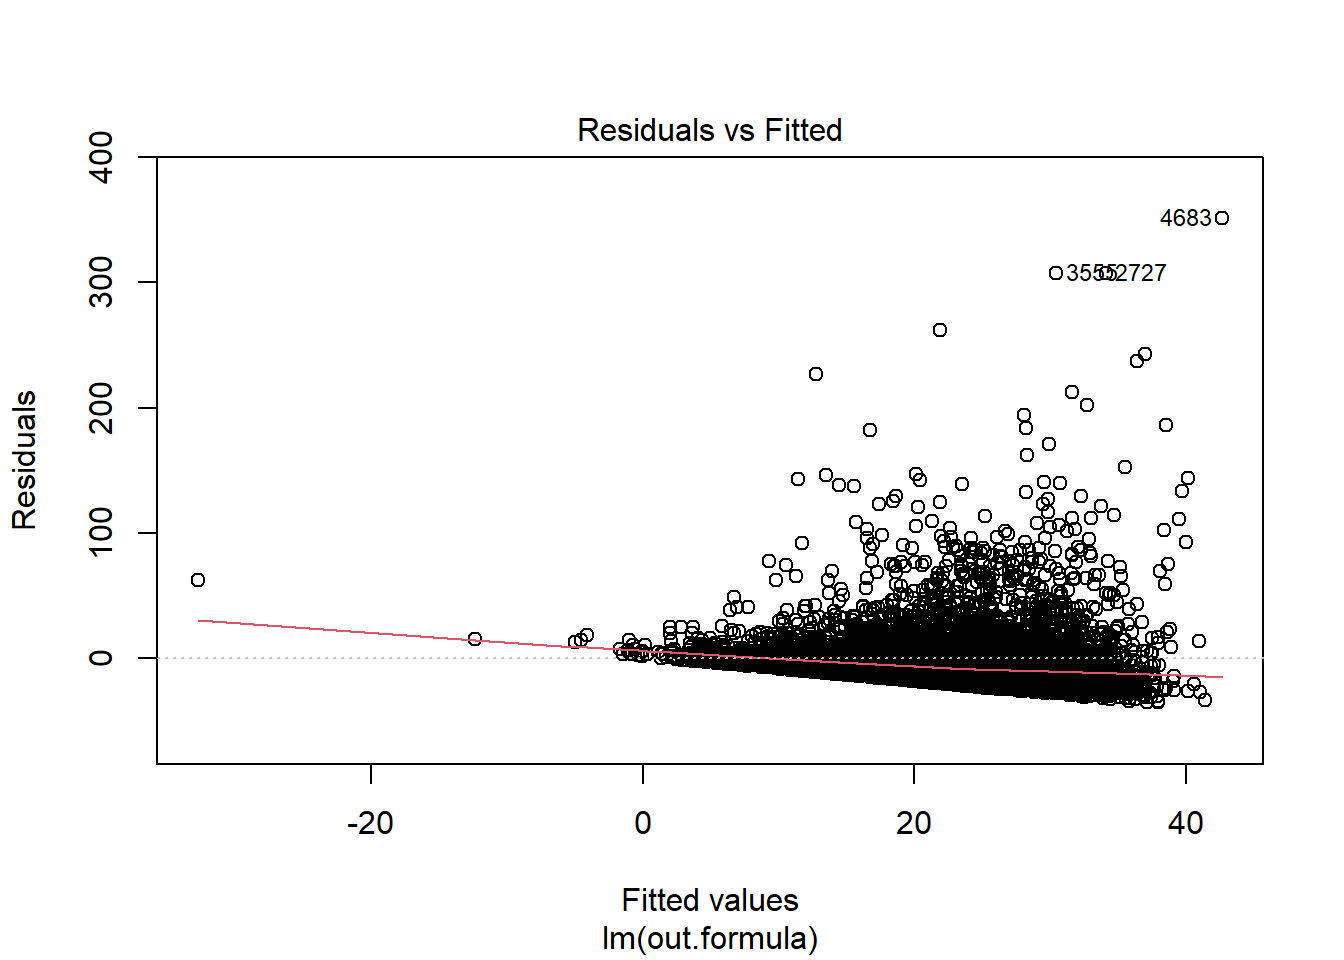
\includegraphics{TMLEw_files/figure-latex/reg2a-1.pdf} 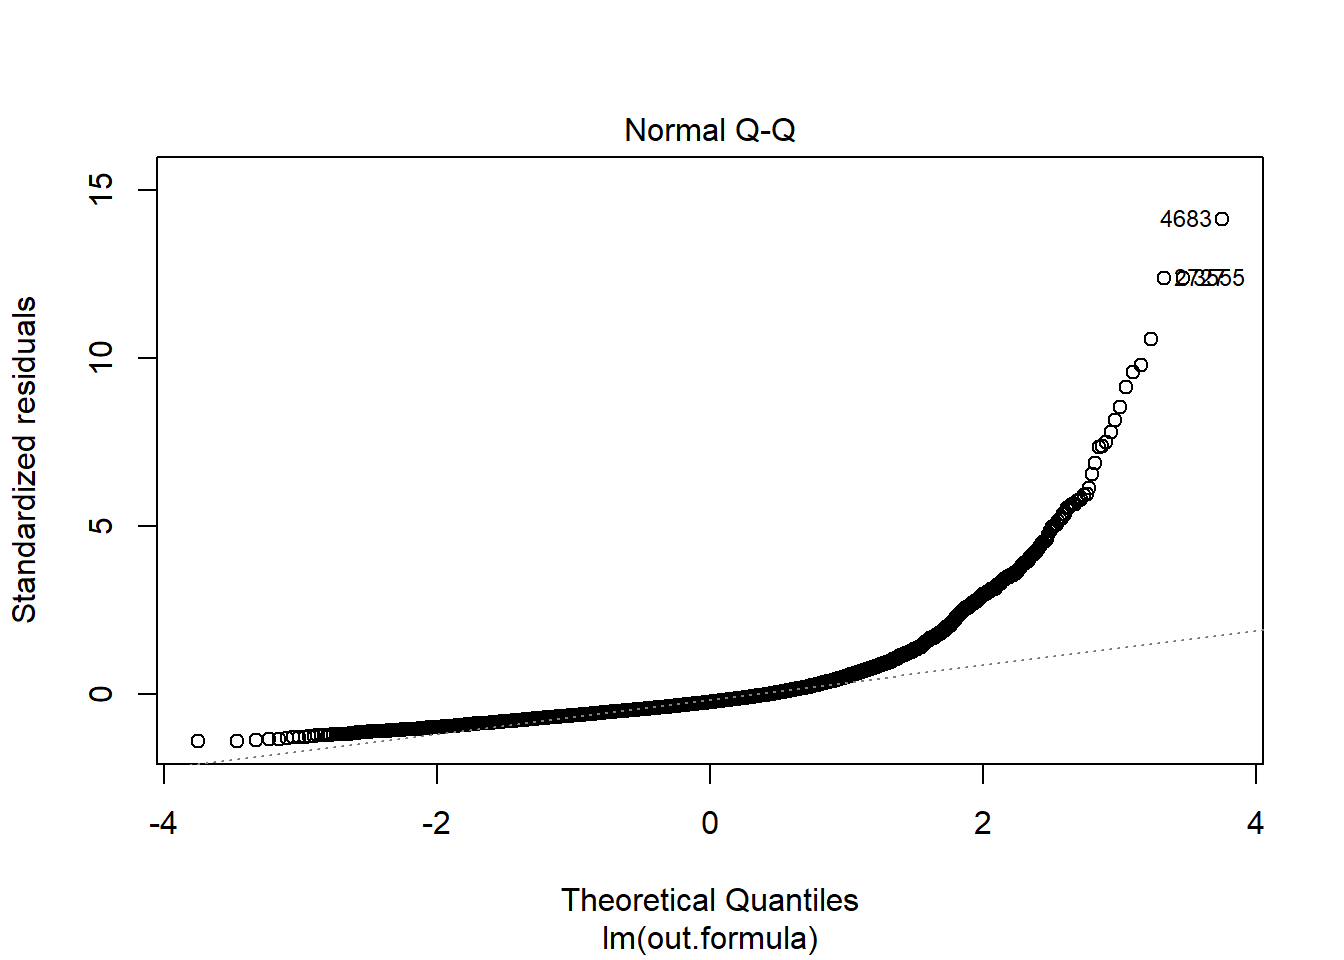
\includegraphics{TMLEw_files/figure-latex/reg2a-2.pdf} 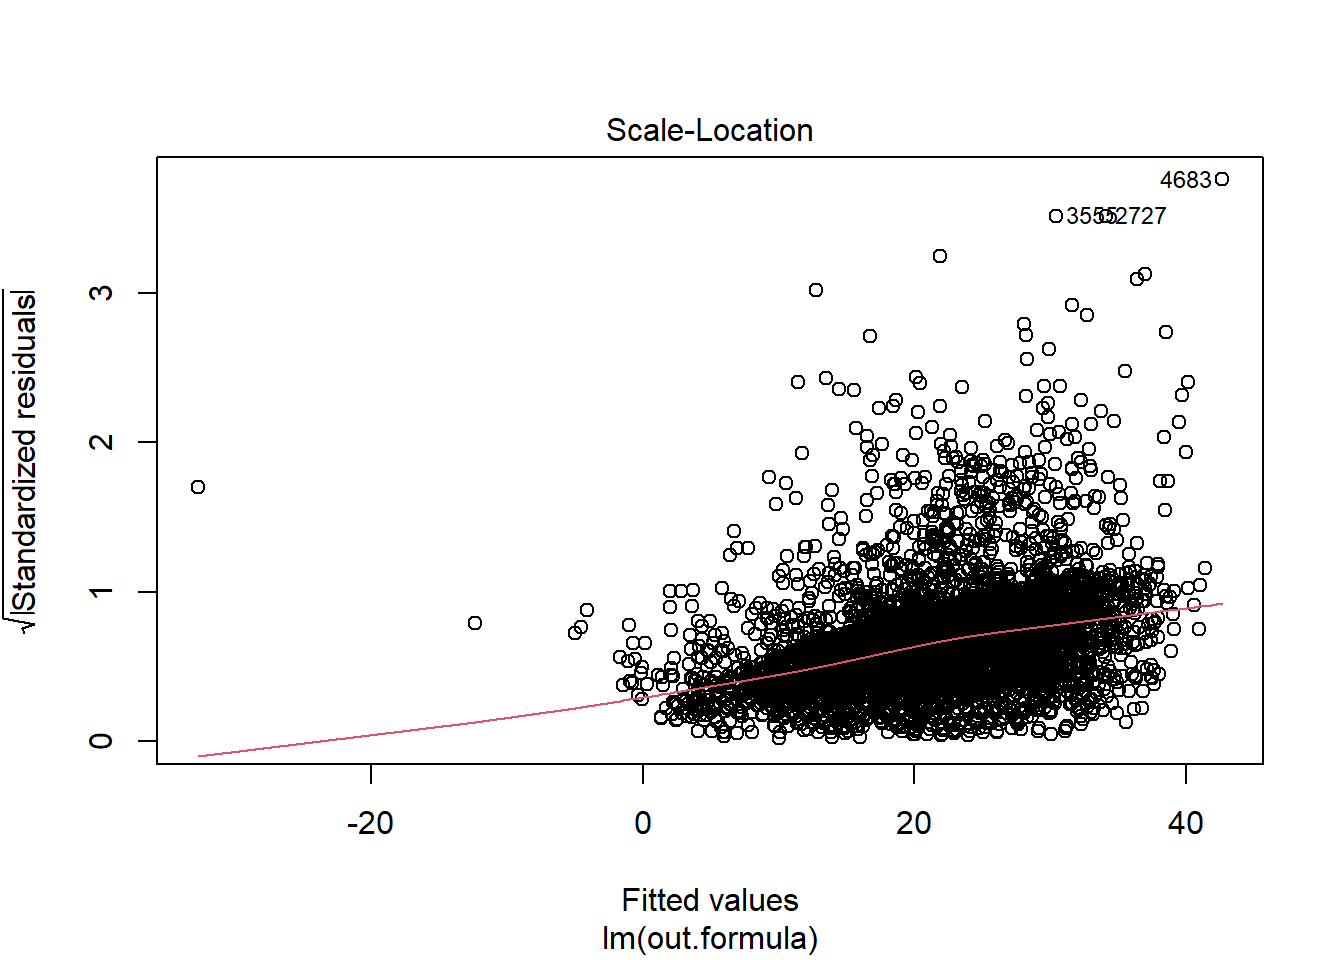
\includegraphics{TMLEw_files/figure-latex/reg2a-3.pdf} 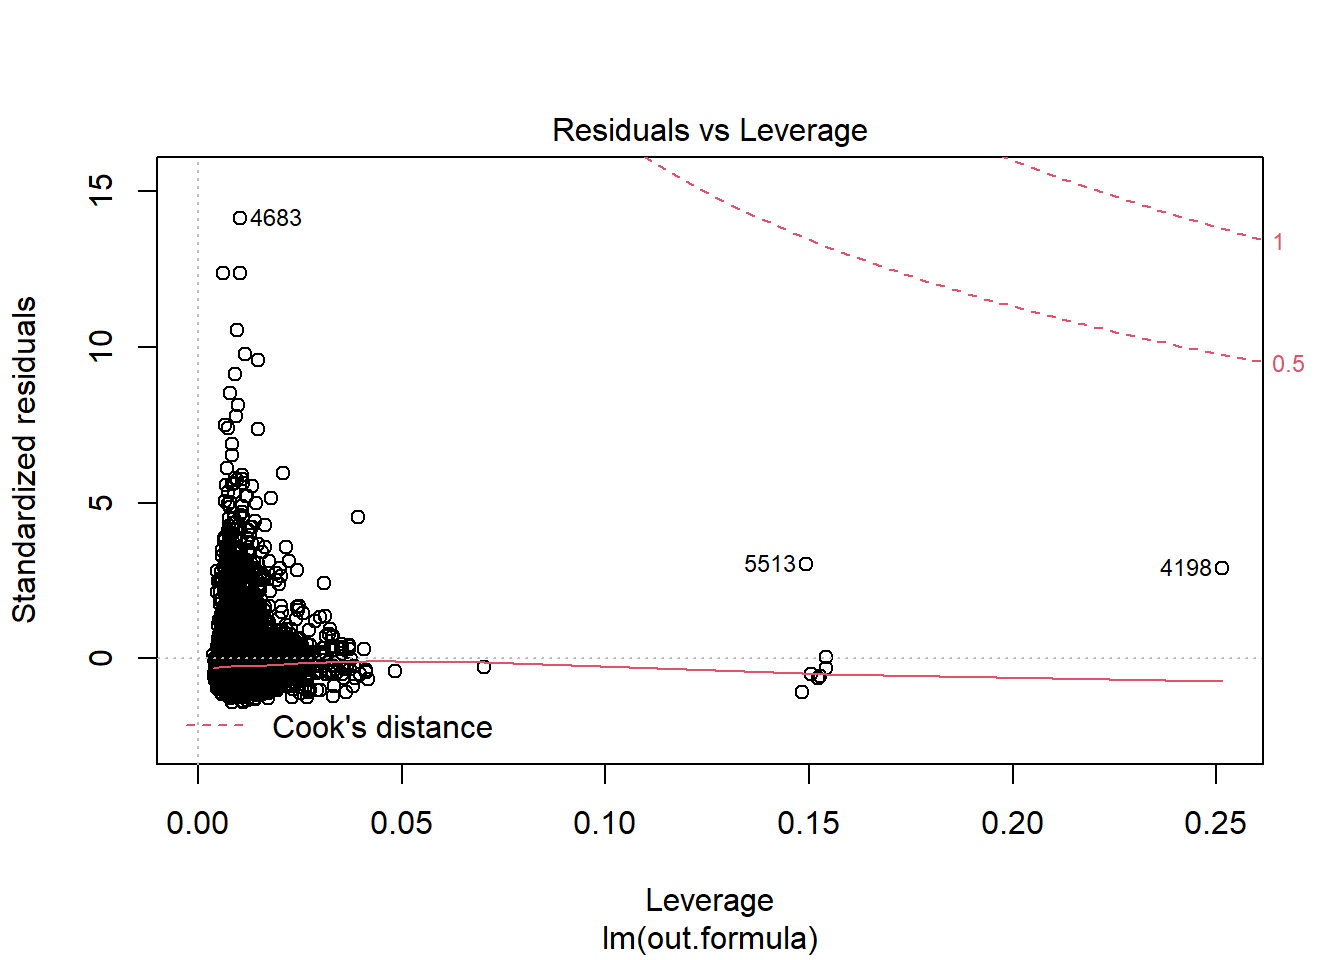
\includegraphics{TMLEw_files/figure-latex/reg2a-4.pdf}

Diagnostics do not necessarily look so good.

\hypertarget{comparison-with-literature}{%
\section{Comparison with literature}\label{comparison-with-literature}}

\citet{connors1996effectiveness} conducted a propensity score matching analysis. Table 5 in \citet{connors1996effectiveness} showed that, after propensity score pair (1-to-1) matching, means of length of stay (\(Y\)), when stratified by RHC (\(A\)) was significantly different.

\hypertarget{psm}{%
\subsection{PSM}\label{psm}}

We also conduct propensity score pair matching analysis, as follows.

\textbf{Note}: In this workshop, we will not cover Propensity Score Matching (PSM) in this workshop. If you want to learn more about this, feel free to check out this other workshop: \href{https://ehsanx.github.io/psw/}{Understanding Propensity Score Matching}.

\begin{Shaded}
\begin{Highlighting}[]
\FunctionTok{set.seed}\NormalTok{(}\DecValTok{123}\NormalTok{)}
\FunctionTok{require}\NormalTok{(MatchIt)}
\NormalTok{ps.formula }\OtherTok{\textless{}{-}} \FunctionTok{as.formula}\NormalTok{(}\FunctionTok{paste}\NormalTok{(}\StringTok{"A\textasciitilde{}"}\NormalTok{, }
                \FunctionTok{paste}\NormalTok{(baselinevars, }\AttributeTok{collapse =} \StringTok{"+"}\NormalTok{)))}
\NormalTok{PS.fit }\OtherTok{\textless{}{-}} \FunctionTok{glm}\NormalTok{(ps.formula,}\AttributeTok{family=}\StringTok{"binomial"}\NormalTok{, }
              \AttributeTok{data=}\NormalTok{ObsData)}
\NormalTok{ObsData}\SpecialCharTok{$}\NormalTok{PS }\OtherTok{\textless{}{-}} \FunctionTok{predict}\NormalTok{(PS.fit, }
                      \AttributeTok{newdata =}\NormalTok{ ObsData, }\AttributeTok{type=}\StringTok{"response"}\NormalTok{)}
\end{Highlighting}
\end{Shaded}

\begin{Shaded}
\begin{Highlighting}[]
\NormalTok{logitPS }\OtherTok{\textless{}{-}}  \SpecialCharTok{{-}}\FunctionTok{log}\NormalTok{(}\DecValTok{1}\SpecialCharTok{/}\NormalTok{ObsData}\SpecialCharTok{$}\NormalTok{PS }\SpecialCharTok{{-}} \DecValTok{1}\NormalTok{) }
\NormalTok{match.obj }\OtherTok{\textless{}{-}} \FunctionTok{matchit}\NormalTok{(ps.formula, }\AttributeTok{data =}\NormalTok{ObsData,}
                     \AttributeTok{distance =}\NormalTok{ ObsData}\SpecialCharTok{$}\NormalTok{PS,}
                     \AttributeTok{method =} \StringTok{"nearest"}\NormalTok{, }\AttributeTok{replace=}\ConstantTok{FALSE}\NormalTok{,}
                     \AttributeTok{ratio =} \DecValTok{1}\NormalTok{, }\AttributeTok{caliper =}\NormalTok{ .}\DecValTok{1}\SpecialCharTok{*}\FunctionTok{sd}\NormalTok{(logitPS))}
\end{Highlighting}
\end{Shaded}

\hypertarget{psm-diagnostics}{%
\subsection{PSM diagnostics}\label{psm-diagnostics}}

\begin{Shaded}
\begin{Highlighting}[]
\FunctionTok{require}\NormalTok{(cobalt)}
\FunctionTok{bal.plot}\NormalTok{(match.obj, }
         \AttributeTok{var.name =} \StringTok{"distance"}\NormalTok{, }
         \AttributeTok{which =} \StringTok{"both"}\NormalTok{,}
         \AttributeTok{type =} \StringTok{"histogram"}\NormalTok{, }
         \AttributeTok{mirror =} \ConstantTok{TRUE}\NormalTok{)}
\end{Highlighting}
\end{Shaded}

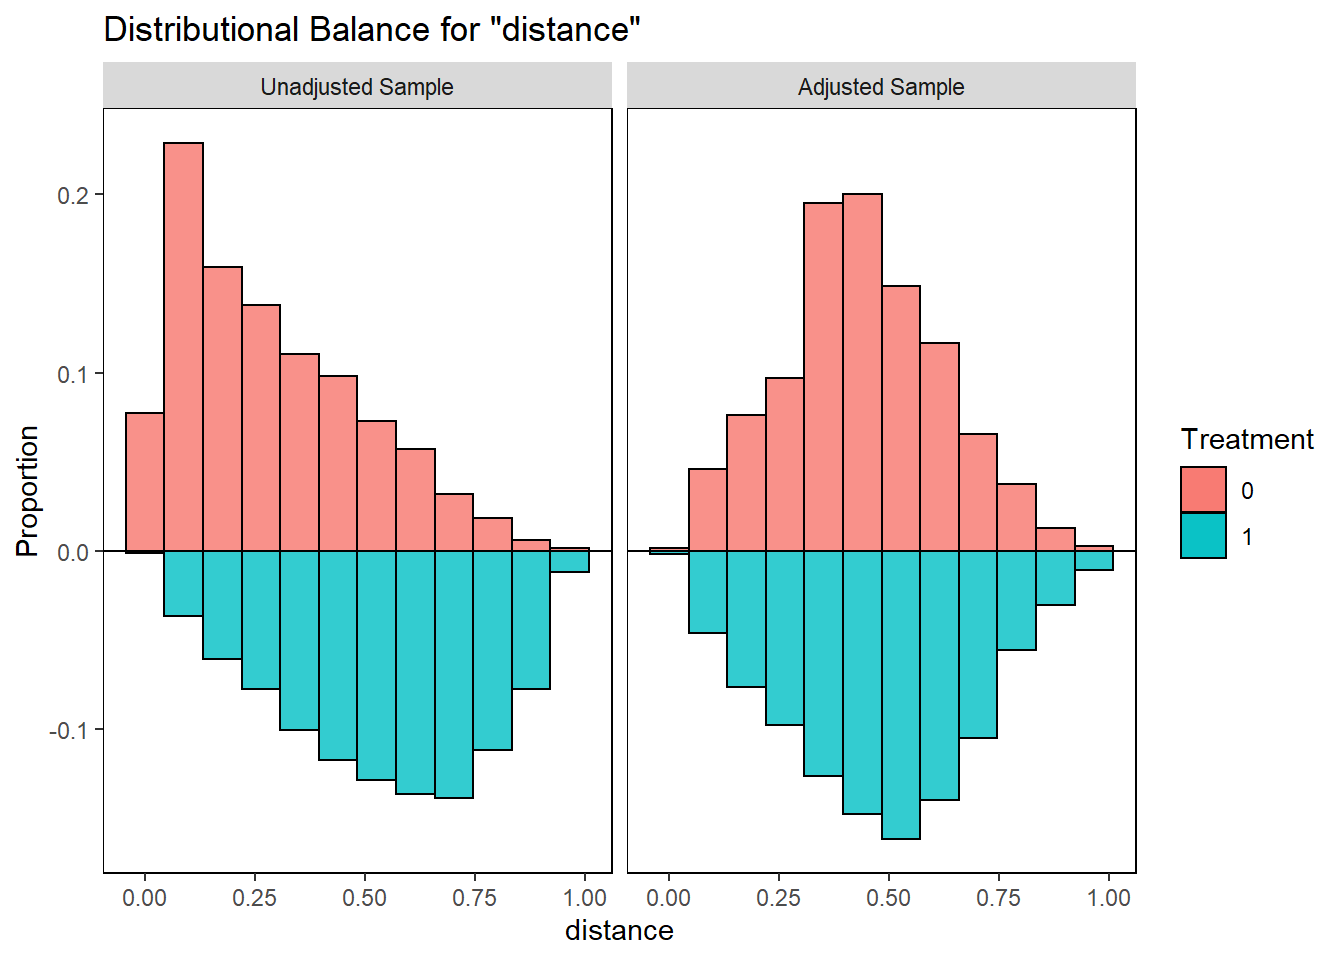
\includegraphics{TMLEw_files/figure-latex/ps2x-1.pdf}

\begin{Shaded}
\begin{Highlighting}[]
\FunctionTok{love.plot}\NormalTok{(match.obj, }\AttributeTok{binary =} \StringTok{"std"}\NormalTok{,}
          \AttributeTok{thresholds =} \FunctionTok{c}\NormalTok{(}\AttributeTok{m =}\NormalTok{ .}\DecValTok{1}\NormalTok{))}
\end{Highlighting}
\end{Shaded}

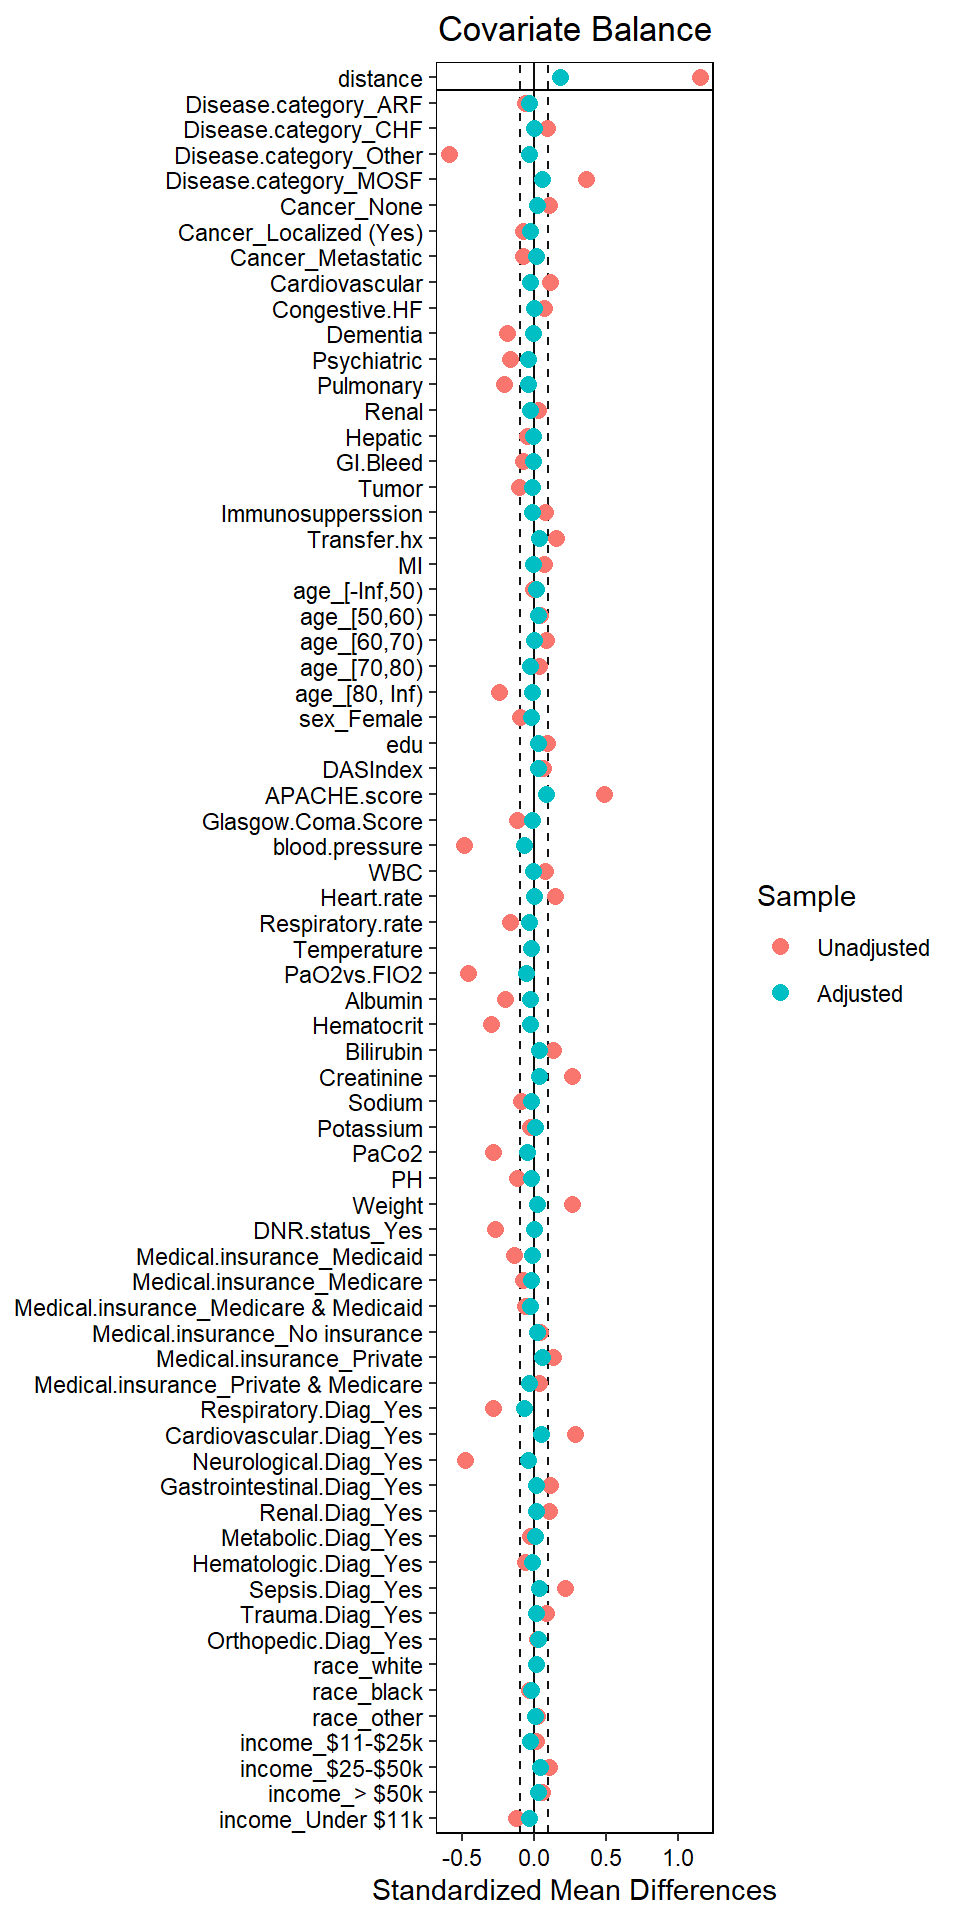
\includegraphics{TMLEw_files/figure-latex/ps2b-1.pdf}

The love plot suggests satisfactory propensity score matching (all SMD \textless{} 0.1).

\hypertarget{psm-results}{%
\subsection{PSM results}\label{psm-results}}

\begin{Shaded}
\begin{Highlighting}[]
\NormalTok{matched.data }\OtherTok{\textless{}{-}} \FunctionTok{match.data}\NormalTok{(match.obj)}
\NormalTok{tab1y }\OtherTok{\textless{}{-}} \FunctionTok{CreateTableOne}\NormalTok{(}\AttributeTok{vars =} \FunctionTok{c}\NormalTok{(}\StringTok{"Y"}\NormalTok{),}
               \AttributeTok{data =}\NormalTok{ matched.data, }\AttributeTok{strata =} \StringTok{"A"}\NormalTok{, }
               \AttributeTok{test =} \ConstantTok{TRUE}\NormalTok{)}
\FunctionTok{print}\NormalTok{(tab1y, }\AttributeTok{showAllLevels =} \ConstantTok{FALSE}\NormalTok{, }
      \AttributeTok{test =} \ConstantTok{TRUE}\NormalTok{) }
\end{Highlighting}
\end{Shaded}

\begin{verbatim}
##                Stratified by A
##                 0             1             p      test
##   n              1628          1628                    
##   Y (mean (SD)) 21.20 (25.58) 24.05 (27.49)  0.002
\end{verbatim}

We also find the same conclusion based on propensity score pair matched data.

\hypertarget{g-computation}{%
\chapter{G-computation}\label{g-computation}}

\hypertarget{closer-look-at-the-data}{%
\section{Closer look at the data}\label{closer-look-at-the-data}}

\begin{Shaded}
\begin{Highlighting}[]
\CommentTok{\# Read the data saved at the last chapter}
\NormalTok{ObsData }\OtherTok{\textless{}{-}} \FunctionTok{readRDS}\NormalTok{(}\AttributeTok{file =} \StringTok{"data/rhcAnalytic.RDS"}\NormalTok{)}
\end{Highlighting}
\end{Shaded}

\hypertarget{view-data-from-6-participants}{%
\subsection{View data from 6 participants}\label{view-data-from-6-participants}}

Let's focus on only first 6 columns.

\begin{Shaded}
\begin{Highlighting}[]
\NormalTok{small.data }\OtherTok{\textless{}{-}}\NormalTok{ ObsData[}\DecValTok{1}\SpecialCharTok{:}\DecValTok{6}\NormalTok{,}\FunctionTok{c}\NormalTok{(}\StringTok{"sex"}\NormalTok{,}\StringTok{"A"}\NormalTok{,}\StringTok{"Y"}\NormalTok{)]}
\FunctionTok{kable}\NormalTok{(small.data)}
\end{Highlighting}
\end{Shaded}

\begin{tabular}{l|r|r}
\hline
sex & A & Y\\
\hline
Male & 0 & 9\\
\hline
Female & 1 & 45\\
\hline
Female & 1 & 60\\
\hline
Female & 0 & 37\\
\hline
Male & 1 & 2\\
\hline
Female & 0 & 7\\
\hline
\end{tabular}

\hypertarget{restructure-the-data-to-estimate-treatment-effect}{%
\subsection{Restructure the data to estimate treatment effect}\label{restructure-the-data-to-estimate-treatment-effect}}

In causal inference literature, often the data is structured in such a way that the outcomes under different treatments are in different columns:

\begin{Shaded}
\begin{Highlighting}[]
\NormalTok{small.data}\SpecialCharTok{$}\NormalTok{id }\OtherTok{\textless{}{-}} \FunctionTok{c}\NormalTok{(}\StringTok{"John"}\NormalTok{,}\StringTok{"Emma"}\NormalTok{,}\StringTok{"Isabella"}\NormalTok{,}\StringTok{"Sophia"}\NormalTok{,}\StringTok{"Luke"}\NormalTok{, }\StringTok{"Mia"}\NormalTok{)}
\NormalTok{small.data}\SpecialCharTok{$}\NormalTok{Y1 }\OtherTok{\textless{}{-}} \FunctionTok{ifelse}\NormalTok{(small.data}\SpecialCharTok{$}\NormalTok{A}\SpecialCharTok{==}\DecValTok{1}\NormalTok{, small.data}\SpecialCharTok{$}\NormalTok{Y, }\ConstantTok{NA}\NormalTok{)}
\NormalTok{small.data}\SpecialCharTok{$}\NormalTok{Y0 }\OtherTok{\textless{}{-}} \FunctionTok{ifelse}\NormalTok{(small.data}\SpecialCharTok{$}\NormalTok{A}\SpecialCharTok{==}\DecValTok{0}\NormalTok{, small.data}\SpecialCharTok{$}\NormalTok{Y, }\ConstantTok{NA}\NormalTok{)}
\NormalTok{small.data}\SpecialCharTok{$}\NormalTok{TE }\OtherTok{\textless{}{-}}\NormalTok{ small.data}\SpecialCharTok{$}\NormalTok{Y1 }\SpecialCharTok{{-}}\NormalTok{ small.data}\SpecialCharTok{$}\NormalTok{Y0}
\NormalTok{small.data }\OtherTok{\textless{}{-}}\NormalTok{ small.data[}\FunctionTok{c}\NormalTok{(}\StringTok{"id"}\NormalTok{, }\StringTok{"sex"}\NormalTok{,}\StringTok{"A"}\NormalTok{,}\StringTok{"Y1"}\NormalTok{,}\StringTok{"Y0"}\NormalTok{, }\StringTok{"TE"}\NormalTok{)]}
\NormalTok{small.data}\SpecialCharTok{$}\NormalTok{Y }\OtherTok{\textless{}{-}} \ConstantTok{NULL}
\NormalTok{small.data}\SpecialCharTok{$}\NormalTok{sex }\OtherTok{\textless{}{-}} \FunctionTok{as.character}\NormalTok{(small.data}\SpecialCharTok{$}\NormalTok{sex)}
\NormalTok{m.Y1 }\OtherTok{\textless{}{-}} \FunctionTok{mean}\NormalTok{(small.data}\SpecialCharTok{$}\NormalTok{Y1, }\AttributeTok{na.rm =} \ConstantTok{TRUE}\NormalTok{)}
\NormalTok{m.Y0 }\OtherTok{\textless{}{-}} \FunctionTok{mean}\NormalTok{(small.data}\SpecialCharTok{$}\NormalTok{Y0, }\AttributeTok{na.rm =} \ConstantTok{TRUE}\NormalTok{)}
\NormalTok{mean.values }\OtherTok{\textless{}{-}} \FunctionTok{round}\NormalTok{(}\FunctionTok{c}\NormalTok{(}\ConstantTok{NA}\NormalTok{,}\ConstantTok{NA}\NormalTok{, }\ConstantTok{NA}\NormalTok{, m.Y1, m.Y0,}
\NormalTok{                 m.Y1 }\SpecialCharTok{{-}}\NormalTok{ m.Y0),}\DecValTok{0}\NormalTok{)}
\NormalTok{small.data2 }\OtherTok{\textless{}{-}} \FunctionTok{rbind}\NormalTok{(small.data, mean.values)}
\FunctionTok{kable}\NormalTok{(small.data2, }\AttributeTok{booktabs =} \ConstantTok{TRUE}\NormalTok{, }\AttributeTok{digits=}\DecValTok{1}\NormalTok{,}
             \AttributeTok{col.names =} \FunctionTok{c}\NormalTok{(}\StringTok{"Subject ID"}\NormalTok{,}\StringTok{"Sex"}\NormalTok{,}
                           \StringTok{"RHC status (A)"}\NormalTok{, }
                           \StringTok{"Y when A=1 (RHC)"}\NormalTok{, }
                           \StringTok{"Y when A=0 (no RHC)"}\NormalTok{, }
                           \StringTok{"Treatment Effect"}\NormalTok{))}\SpecialCharTok{\%\textgreater{}\%}
  \FunctionTok{row\_spec}\NormalTok{(}\DecValTok{7}\NormalTok{, }\AttributeTok{bold =} \ConstantTok{TRUE}\NormalTok{, }\AttributeTok{color =} \StringTok{"white"}\NormalTok{, }
           \AttributeTok{background =} \StringTok{"\#D7261E"}\NormalTok{)}
\end{Highlighting}
\end{Shaded}

\begin{tabular}{llrrrr}
\toprule
Subject ID & Sex & RHC status (A) & Y when A=1 (RHC) & Y when A=0 (no RHC) & Treatment Effect\\
\midrule
John & Male & 0 &  & 9 & \\
Emma & Female & 1 & 45 &  & \\
Isabella & Female & 1 & 60 &  & \\
Sophia & Female & 0 &  & 37 & \\
Luke & Male & 1 & 2 &  & \\
\addlinespace
Mia & Female & 0 &  & 7 & \\
\cellcolor[HTML]{D7261E}{\textcolor{white}{\textbf{}}} & \cellcolor[HTML]{D7261E}{\textcolor{white}{\textbf{}}} & \cellcolor[HTML]{D7261E}{\textcolor{white}{\textbf{}}} & \cellcolor[HTML]{D7261E}{\textcolor{white}{\textbf{36}}} & \cellcolor[HTML]{D7261E}{\textcolor{white}{\textbf{18}}} & \cellcolor[HTML]{D7261E}{\textcolor{white}{\textbf{18}}}\\
\bottomrule
\end{tabular}

Then it is easy to see

\begin{itemize}
\tightlist
\item
  the mean outcome under treated group (\texttt{RHC})
\item
  the mean outcome under untreated group (\texttt{no\ RHC})
\end{itemize}

and the difference between these two means are the treatment effect.

\hypertarget{treat-the-problem-as-a-missing-value-problem}{%
\subsection{Treat the problem as a missing value problem}\label{treat-the-problem-as-a-missing-value-problem}}

Instead of just estimating treatment effect on an average level, an alternate could be to

\begin{itemize}
\tightlist
\item
  impute mean outcomes for the treated subjects
\item
  impute mean outcomes for the untreated subjects
\item
  Calculate individual treatment effect estimate
\item
  then calculate the average treatment effect
\end{itemize}

\begin{Shaded}
\begin{Highlighting}[]
\NormalTok{small.data0 }\OtherTok{\textless{}{-}}\NormalTok{ small.data}
\NormalTok{small.data}\SpecialCharTok{$}\NormalTok{Y1[}\FunctionTok{is.na}\NormalTok{(small.data}\SpecialCharTok{$}\NormalTok{Y1)] }\OtherTok{\textless{}{-}} \FunctionTok{round}\NormalTok{(m.Y1)}
\NormalTok{small.data}\SpecialCharTok{$}\NormalTok{Y0[}\FunctionTok{is.na}\NormalTok{(small.data}\SpecialCharTok{$}\NormalTok{Y0)] }\OtherTok{\textless{}{-}} \FunctionTok{round}\NormalTok{(m.Y0)}
\NormalTok{small.data}\SpecialCharTok{$}\NormalTok{TE }\OtherTok{\textless{}{-}}\NormalTok{ small.data}\SpecialCharTok{$}\NormalTok{Y1 }\SpecialCharTok{{-}}\NormalTok{ small.data}\SpecialCharTok{$}\NormalTok{Y0}
\NormalTok{m.Y1 }\OtherTok{\textless{}{-}} \FunctionTok{mean}\NormalTok{(small.data}\SpecialCharTok{$}\NormalTok{Y1)}
\NormalTok{m.Y0 }\OtherTok{\textless{}{-}} \FunctionTok{mean}\NormalTok{(small.data}\SpecialCharTok{$}\NormalTok{Y0)}
\NormalTok{m.TE }\OtherTok{\textless{}{-}} \FunctionTok{mean}\NormalTok{(small.data}\SpecialCharTok{$}\NormalTok{TE)}
\NormalTok{mean.values }\OtherTok{\textless{}{-}} \FunctionTok{round}\NormalTok{(}\FunctionTok{c}\NormalTok{(}\ConstantTok{NA}\NormalTok{,}\ConstantTok{NA}\NormalTok{, }\ConstantTok{NA}\NormalTok{, m.Y1, m.Y0, m.TE),}\DecValTok{0}\NormalTok{)}
\NormalTok{small.data2 }\OtherTok{\textless{}{-}} \FunctionTok{rbind}\NormalTok{(small.data, mean.values)}
\FunctionTok{kable}\NormalTok{(small.data2, }\AttributeTok{booktabs =} \ConstantTok{TRUE}\NormalTok{, }\AttributeTok{digits=}\DecValTok{1}\NormalTok{,}
             \AttributeTok{col.names =} \FunctionTok{c}\NormalTok{(}\StringTok{"Subject ID"}\NormalTok{,}\StringTok{"Sex"}\NormalTok{,}
                           \StringTok{"RHC status (A)"}\NormalTok{, }
                           \StringTok{"Y when A=1 (RHC)"}\NormalTok{, }
                           \StringTok{"Y when A=0 (no RHC)"}\NormalTok{, }
                           \StringTok{"Treatment Effect"}\NormalTok{))}\SpecialCharTok{\%\textgreater{}\%}
  \FunctionTok{row\_spec}\NormalTok{(}\DecValTok{7}\NormalTok{, }\AttributeTok{bold =} \ConstantTok{TRUE}\NormalTok{, }\AttributeTok{color =} \StringTok{"white"}\NormalTok{, }
           \AttributeTok{background =} \StringTok{"\#D7261E"}\NormalTok{)}
\end{Highlighting}
\end{Shaded}

\begin{tabular}{llrrrr}
\toprule
Subject ID & Sex & RHC status (A) & Y when A=1 (RHC) & Y when A=0 (no RHC) & Treatment Effect\\
\midrule
John & Male & 0 & 36 & 9 & 27\\
Emma & Female & 1 & 45 & 18 & 27\\
Isabella & Female & 1 & 60 & 18 & 42\\
Sophia & Female & 0 & 36 & 37 & -1\\
Luke & Male & 1 & 2 & 18 & -16\\
\addlinespace
Mia & Female & 0 & 36 & 7 & 29\\
\cellcolor[HTML]{D7261E}{\textcolor{white}{\textbf{}}} & \cellcolor[HTML]{D7261E}{\textcolor{white}{\textbf{}}} & \cellcolor[HTML]{D7261E}{\textcolor{white}{\textbf{}}} & \cellcolor[HTML]{D7261E}{\textcolor{white}{\textbf{36}}} & \cellcolor[HTML]{D7261E}{\textcolor{white}{\textbf{18}}} & \cellcolor[HTML]{D7261E}{\textcolor{white}{\textbf{18}}}\\
\bottomrule
\end{tabular}

\hypertarget{impute-better-value}{%
\subsection{Impute better value?}\label{impute-better-value}}

However, assume that the effect of the treatment for male and female are not the same. Then, it might make more sense to impute means specific to males for male subjects, and separately impute means specific to females for female subjects.

\begin{Shaded}
\begin{Highlighting}[]
\NormalTok{small.data }\OtherTok{\textless{}{-}}\NormalTok{ small.data0}
\NormalTok{m.Y1m }\OtherTok{\textless{}{-}} \FunctionTok{mean}\NormalTok{(small.data}\SpecialCharTok{$}\NormalTok{Y1[small.data}\SpecialCharTok{$}\NormalTok{sex }\SpecialCharTok{==} \StringTok{"Male"}\NormalTok{], }\AttributeTok{na.rm =} \ConstantTok{TRUE}\NormalTok{)}
\NormalTok{m.Y1f }\OtherTok{\textless{}{-}} \FunctionTok{mean}\NormalTok{(small.data}\SpecialCharTok{$}\NormalTok{Y1[small.data}\SpecialCharTok{$}\NormalTok{sex }\SpecialCharTok{==} \StringTok{"Female"}\NormalTok{], }\AttributeTok{na.rm =} \ConstantTok{TRUE}\NormalTok{)}
\NormalTok{m.Y0m }\OtherTok{\textless{}{-}} \FunctionTok{mean}\NormalTok{(small.data}\SpecialCharTok{$}\NormalTok{Y0[small.data}\SpecialCharTok{$}\NormalTok{sex }\SpecialCharTok{==} \StringTok{"Male"}\NormalTok{], }\AttributeTok{na.rm =} \ConstantTok{TRUE}\NormalTok{)}
\NormalTok{m.Y0f }\OtherTok{\textless{}{-}} \FunctionTok{mean}\NormalTok{(small.data}\SpecialCharTok{$}\NormalTok{Y0[small.data}\SpecialCharTok{$}\NormalTok{sex }\SpecialCharTok{==} \StringTok{"Female"}\NormalTok{], }\AttributeTok{na.rm =} \ConstantTok{TRUE}\NormalTok{)}
\NormalTok{m.TE.m }\OtherTok{\textless{}{-}}\NormalTok{ m.Y1m}\SpecialCharTok{{-}}\NormalTok{m.Y0m}
\NormalTok{m.TE.f }\OtherTok{\textless{}{-}}\NormalTok{ m.Y1f}\SpecialCharTok{{-}}\NormalTok{m.Y0f}
\NormalTok{mean.values.m }\OtherTok{\textless{}{-}} \FunctionTok{round}\NormalTok{(}\FunctionTok{c}\NormalTok{(}\ConstantTok{NA}\NormalTok{,}\ConstantTok{NA}\NormalTok{, }\ConstantTok{NA}\NormalTok{, m.Y1m, m.Y0m, m.TE.m),}\DecValTok{0}\NormalTok{)}
\NormalTok{mean.values.f }\OtherTok{\textless{}{-}} \FunctionTok{round}\NormalTok{(}\FunctionTok{c}\NormalTok{(}\ConstantTok{NA}\NormalTok{,}\ConstantTok{NA}\NormalTok{, }\ConstantTok{NA}\NormalTok{, m.Y1f, m.Y0f, m.TE.f),}\DecValTok{0}\NormalTok{)}
\NormalTok{small.data}\SpecialCharTok{$}\NormalTok{Y1[small.data}\SpecialCharTok{$}\NormalTok{sex }\SpecialCharTok{==} 
                \StringTok{"Male"}\NormalTok{][}\FunctionTok{is.na}\NormalTok{(small.data}\SpecialCharTok{$}\NormalTok{Y1[small.data}\SpecialCharTok{$}\NormalTok{sex }\SpecialCharTok{==} 
                                              \StringTok{"Male"}\NormalTok{])] }\OtherTok{\textless{}{-}} \FunctionTok{round}\NormalTok{(m.Y1m)}
\NormalTok{small.data}\SpecialCharTok{$}\NormalTok{Y0[small.data}\SpecialCharTok{$}\NormalTok{sex }\SpecialCharTok{==} 
                \StringTok{"Male"}\NormalTok{][}\FunctionTok{is.na}\NormalTok{(small.data}\SpecialCharTok{$}\NormalTok{Y0[small.data}\SpecialCharTok{$}\NormalTok{sex }\SpecialCharTok{==} 
                                              \StringTok{"Male"}\NormalTok{])] }\OtherTok{\textless{}{-}} \FunctionTok{round}\NormalTok{(m.Y0m)}
\NormalTok{small.data}\SpecialCharTok{$}\NormalTok{Y1[small.data}\SpecialCharTok{$}\NormalTok{sex }\SpecialCharTok{==} 
                \StringTok{"Female"}\NormalTok{][}\FunctionTok{is.na}\NormalTok{(small.data}\SpecialCharTok{$}\NormalTok{Y1[small.data}\SpecialCharTok{$}\NormalTok{sex }\SpecialCharTok{==} 
                                                \StringTok{"Female"}\NormalTok{])] }\OtherTok{\textless{}{-}} \FunctionTok{round}\NormalTok{(m.Y1f)}
\NormalTok{small.data}\SpecialCharTok{$}\NormalTok{Y0[small.data}\SpecialCharTok{$}\NormalTok{sex }\SpecialCharTok{==} 
                \StringTok{"Female"}\NormalTok{][}\FunctionTok{is.na}\NormalTok{(small.data}\SpecialCharTok{$}\NormalTok{Y0[small.data}\SpecialCharTok{$}\NormalTok{sex }\SpecialCharTok{==} 
                                                \StringTok{"Female"}\NormalTok{])] }\OtherTok{\textless{}{-}} \FunctionTok{round}\NormalTok{(m.Y0f)}
\NormalTok{small.data}\SpecialCharTok{$}\NormalTok{TE }\OtherTok{\textless{}{-}}\NormalTok{ small.data}\SpecialCharTok{$}\NormalTok{Y1 }\SpecialCharTok{{-}}\NormalTok{ small.data}\SpecialCharTok{$}\NormalTok{Y0}
\NormalTok{small.data2 }\OtherTok{\textless{}{-}} \FunctionTok{rbind}\NormalTok{(small.data, mean.values.m,mean.values.f)}
\FunctionTok{kable}\NormalTok{(small.data2, }\AttributeTok{booktabs =} \ConstantTok{TRUE}\NormalTok{, }\AttributeTok{digits=}\DecValTok{1}\NormalTok{,}
             \AttributeTok{col.names =} \FunctionTok{c}\NormalTok{(}\StringTok{"Subject ID"}\NormalTok{,}\StringTok{"Sex"}\NormalTok{,}\StringTok{"RHC status (A)"}\NormalTok{, }
                           \StringTok{"Y when A=1 (RHC)"}\NormalTok{, }\StringTok{"Y when A=0 (no RHC)"}\NormalTok{, }
                           \StringTok{"Treatment Effect"}\NormalTok{))}\SpecialCharTok{\%\textgreater{}\%}
  \FunctionTok{row\_spec}\NormalTok{(}\DecValTok{7}\NormalTok{, }\AttributeTok{bold =} \ConstantTok{TRUE}\NormalTok{, }\AttributeTok{color =} \StringTok{"white"}\NormalTok{, }\AttributeTok{background =} \StringTok{"\#D7261E"}\NormalTok{)}\SpecialCharTok{\%\textgreater{}\%}
  \FunctionTok{row\_spec}\NormalTok{(}\DecValTok{8}\NormalTok{, }\AttributeTok{bold =} \ConstantTok{TRUE}\NormalTok{, }\AttributeTok{color =} \StringTok{"white"}\NormalTok{, }\AttributeTok{background =} \StringTok{"\#D7261E"}\NormalTok{)}
\end{Highlighting}
\end{Shaded}

\begin{tabular}{llrrrr}
\toprule
Subject ID & Sex & RHC status (A) & Y when A=1 (RHC) & Y when A=0 (no RHC) & Treatment Effect\\
\midrule
John & Male & 0 & 2 & 9 & -7\\
Emma & Female & 1 & 45 & 22 & 23\\
Isabella & Female & 1 & 60 & 22 & 38\\
Sophia & Female & 0 & 52 & 37 & 15\\
Luke & Male & 1 & 2 & 9 & -7\\
\addlinespace
Mia & Female & 0 & 52 & 7 & 45\\
\cellcolor[HTML]{D7261E}{\textcolor{white}{\textbf{}}} & \cellcolor[HTML]{D7261E}{\textcolor{white}{\textbf{}}} & \cellcolor[HTML]{D7261E}{\textcolor{white}{\textbf{}}} & \cellcolor[HTML]{D7261E}{\textcolor{white}{\textbf{2}}} & \cellcolor[HTML]{D7261E}{\textcolor{white}{\textbf{9}}} & \cellcolor[HTML]{D7261E}{\textcolor{white}{\textbf{-7}}}\\
\cellcolor[HTML]{D7261E}{\textcolor{white}{\textbf{}}} & \cellcolor[HTML]{D7261E}{\textcolor{white}{\textbf{}}} & \cellcolor[HTML]{D7261E}{\textcolor{white}{\textbf{}}} & \cellcolor[HTML]{D7261E}{\textcolor{white}{\textbf{52}}} & \cellcolor[HTML]{D7261E}{\textcolor{white}{\textbf{22}}} & \cellcolor[HTML]{D7261E}{\textcolor{white}{\textbf{30}}}\\
\bottomrule
\end{tabular}

\begin{itemize}
\tightlist
\item
  Extending the problem to other covariates, you can see that we could condition on rest of the covariates (such as age, income, race, disease category) to get better imputation values.
\item
  Regression is a generalized method to take mean conditional on many covariates.
\end{itemize}

\hypertarget{use-regression-for-predicting-outcome}{%
\section{Use Regression for predicting outcome}\label{use-regression-for-predicting-outcome}}

Let us fit the outcome with all covariates, including the exposure status.

\begin{Shaded}
\begin{Highlighting}[]
\CommentTok{\# isolate the names of baseline covariates}
\NormalTok{baselinevars }\OtherTok{\textless{}{-}} \FunctionTok{names}\NormalTok{(dplyr}\SpecialCharTok{::}\FunctionTok{select}\NormalTok{(ObsData, }\SpecialCharTok{!}\FunctionTok{c}\NormalTok{(A,Y)))}
\CommentTok{\# adjust the exposure variable (primary interest) + covariates}
\NormalTok{out.formula }\OtherTok{\textless{}{-}} \FunctionTok{as.formula}\NormalTok{(}\FunctionTok{paste}\NormalTok{(}\StringTok{"Y\textasciitilde{} A +"}\NormalTok{, }
                               \FunctionTok{paste}\NormalTok{(baselinevars, }
                                     \AttributeTok{collapse =} \StringTok{"+"}\NormalTok{)))}
\NormalTok{fit1 }\OtherTok{\textless{}{-}} \FunctionTok{lm}\NormalTok{(out.formula, }\AttributeTok{data =}\NormalTok{ ObsData)}
\FunctionTok{coef}\NormalTok{(fit1)}
\end{Highlighting}
\end{Shaded}

\begin{verbatim}
##                          (Intercept)                                    A 
##                        -7.680847e+01                         2.902030e+00 
##                  Disease.categoryCHF                Disease.categoryOther 
##                        -5.594331e+00                        -4.421893e+00 
##                 Disease.categoryMOSF                CancerLocalized (Yes) 
##                         2.873451e+00                        -7.794459e+00 
##                     CancerMetastatic                      Cardiovascular1 
##                        -1.056549e+01                         6.605038e-01 
##                       Congestive.HF1                            Dementia1 
##                        -1.754818e+00                        -1.261136e+00 
##                         Psychiatric1                           Pulmonary1 
##                        -4.841489e-01                         2.063282e+00 
##                               Renal1                             Hepatic1 
##                        -6.935923e+00                        -1.523238e+00 
##                            GI.Bleed1                               Tumor1 
##                        -5.096253e+00                         4.573818e+00 
##                   Immunosupperssion1                         Transfer.hx1 
##                         1.103694e-01                         1.161342e+00 
##                                  MI1                           age[50,60) 
##                        -1.650935e+00                         1.429833e-01 
##                           age[60,70)                           age[70,80) 
##                        -4.055267e-01                        -1.103439e+00 
##                         age[80, Inf)                            sexFemale 
##                        -2.757278e+00                         8.272236e-01 
##                                  edu                             DASIndex 
##                         4.775891e-02                        -5.343588e-02 
##                         APACHE.score                   Glasgow.Coma.Score 
##                        -7.020692e-02                         1.563055e-02 
##                       blood.pressure                                  WBC 
##                        -1.323182e-02                         3.940879e-02 
##                           Heart.rate                     Respiratory.rate 
##                         2.244431e-02                        -1.467861e-03 
##                          Temperature                          PaO2vs.FIO2 
##                         5.086475e-01                        -8.517735e-03 
##                              Albumin                           Hematocrit 
##                        -2.570965e+00                        -1.951544e-01 
##                            Bilirubin                           Creatinine 
##                        -9.814574e-02                         5.210509e-01 
##                               Sodium                            Potassium 
##                         1.365534e-01                         3.447162e-01 
##                                PaCo2                                   PH 
##                         1.165866e-01                         1.005261e+01 
##                               Weight                        DNR.statusYes 
##                         2.257116e-04                        -7.959037e+00 
##            Medical.insuranceMedicare Medical.insuranceMedicare & Medicaid 
##                        -5.174593e-01                        -2.422199e+00 
##        Medical.insuranceNo insurance             Medical.insurancePrivate 
##                        -1.785085e+00                        -2.086480e+00 
##  Medical.insurancePrivate & Medicare                  Respiratory.DiagYes 
##                        -2.018369e+00                         3.404743e-01 
##               Cardiovascular.DiagYes                 Neurological.DiagYes 
##                         3.784972e-01                         3.541516e+00 
##             Gastrointestinal.DiagYes                        Renal.DiagYes 
##                         2.551541e+00                         1.784893e+00 
##                    Metabolic.DiagYes                  Hematologic.DiagYes 
##                        -1.161415e+00                        -3.858024e+00 
##                       Sepsis.DiagYes                       Trauma.DiagYes 
##                         2.716148e-03                         1.112049e+00 
##                   Orthopedic.DiagYes                            raceblack 
##                         3.543464e+00                        -1.149936e+00 
##                            raceother                       income$25-$50k 
##                         2.467487e-01                         2.459547e+00 
##                         income> $50k                     incomeUnder $11k 
##                         4.214815e-01                        -4.284414e-01
\end{verbatim}

\hypertarget{predict-outcome-for-treated}{%
\subsection{Predict outcome for treated}\label{predict-outcome-for-treated}}

\begin{itemize}
\tightlist
\item
  Using the regression fit, we can obtain predicted outcome values for the treated.
\item
  We are not only predicting for the unobserved, but also for the observed values when a person was treated.
\end{itemize}

\begin{Shaded}
\begin{Highlighting}[]
\NormalTok{ObsData}\SpecialCharTok{$}\NormalTok{Pred.Y1 }\OtherTok{\textless{}{-}} \FunctionTok{predict}\NormalTok{(fit1, }
                           \AttributeTok{newdata =} \FunctionTok{data.frame}\NormalTok{(}\AttributeTok{A =} \DecValTok{1}\NormalTok{, }
\NormalTok{                                                dplyr}\SpecialCharTok{::}\FunctionTok{select}\NormalTok{(ObsData, }\SpecialCharTok{!}\FunctionTok{c}\NormalTok{(A,Y))), }
                           \AttributeTok{type =} \StringTok{"response"}\NormalTok{)}
\FunctionTok{mean}\NormalTok{(ObsData}\SpecialCharTok{$}\NormalTok{Pred.Y1)}
\end{Highlighting}
\end{Shaded}

\begin{verbatim}
## [1] 23.35625
\end{verbatim}

\begin{Shaded}
\begin{Highlighting}[]
\FunctionTok{hist}\NormalTok{(ObsData}\SpecialCharTok{$}\NormalTok{Pred.Y1, }
     \AttributeTok{main =} \StringTok{"Histogram for predicted outcome for treated"}\NormalTok{, }
     \AttributeTok{xlab =} \StringTok{"Y(A=1)"}\NormalTok{)}
\FunctionTok{abline}\NormalTok{(}\AttributeTok{v=}\FunctionTok{mean}\NormalTok{(ObsData}\SpecialCharTok{$}\NormalTok{Pred.Y1),}\AttributeTok{col=}\StringTok{"blue"}\NormalTok{, }\AttributeTok{lwd =} \DecValTok{4}\NormalTok{)}
\end{Highlighting}
\end{Shaded}

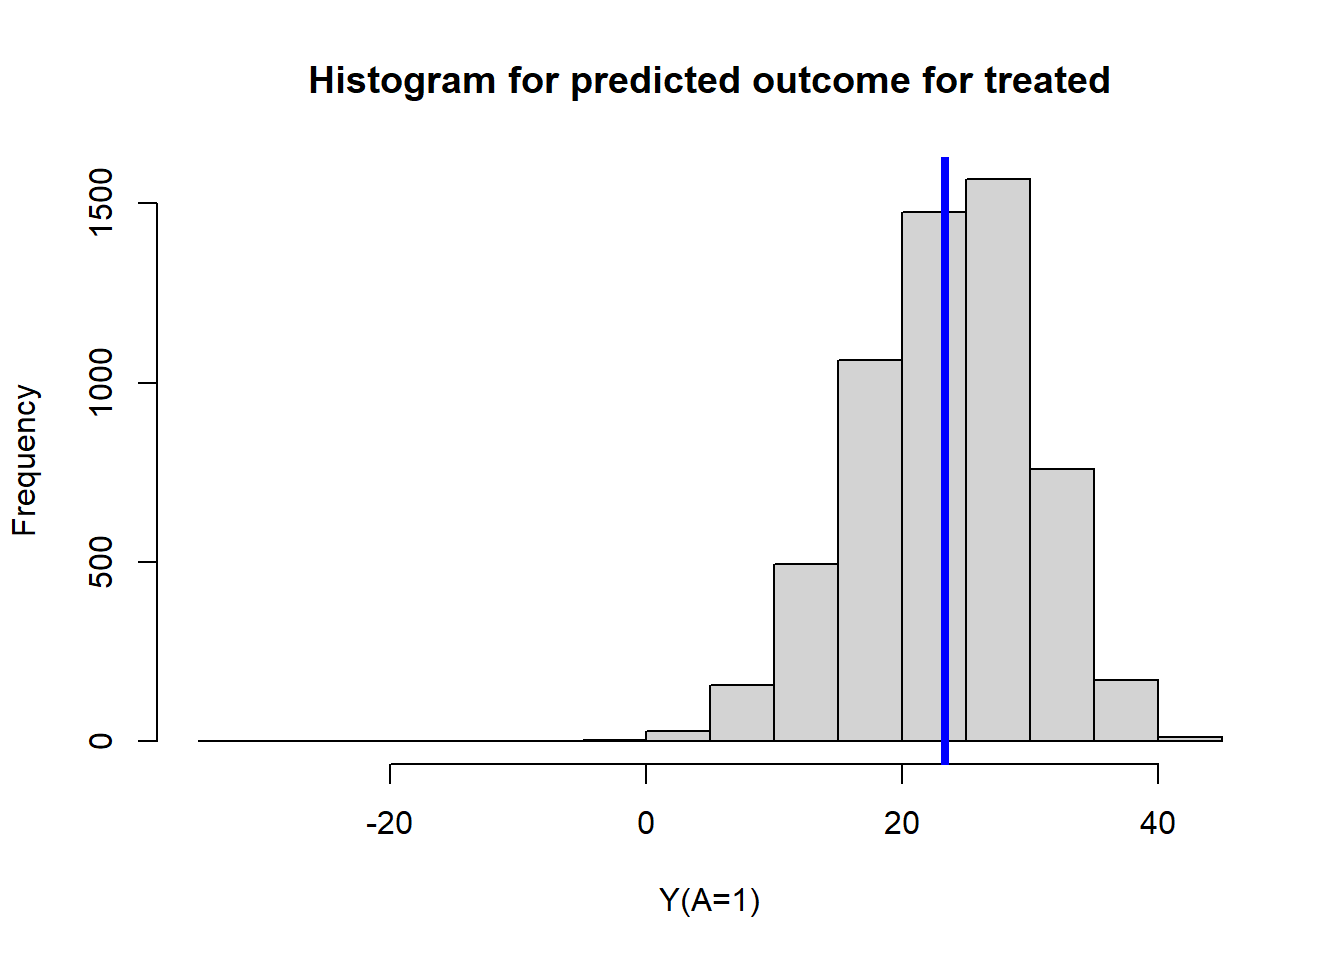
\includegraphics{TMLEw_files/figure-latex/reg2ab-1.pdf}

\hypertarget{look-at-the-predicted-outcome-data-for-treated}{%
\subsection{Look at the predicted outcome data for treated}\label{look-at-the-predicted-outcome-data-for-treated}}

\begin{Shaded}
\begin{Highlighting}[]
\NormalTok{small.data1 }\OtherTok{\textless{}{-}}\NormalTok{ ObsData[}\DecValTok{1}\SpecialCharTok{:}\DecValTok{6}\NormalTok{,}\FunctionTok{c}\NormalTok{(}\StringTok{"A"}\NormalTok{,}\StringTok{"Pred.Y1"}\NormalTok{)]}
\NormalTok{small.data1}\SpecialCharTok{$}\NormalTok{id }\OtherTok{\textless{}{-}} \FunctionTok{c}\NormalTok{(}\StringTok{"John"}\NormalTok{,}\StringTok{"Emma"}\NormalTok{,}\StringTok{"Isabella"}\NormalTok{,}\StringTok{"Sophia"}\NormalTok{,}\StringTok{"Luke"}\NormalTok{, }\StringTok{"Mia"}\NormalTok{)}
\NormalTok{small.data1 }\OtherTok{\textless{}{-}}\NormalTok{ small.data1[}\FunctionTok{c}\NormalTok{(}\StringTok{"id"}\NormalTok{, }\StringTok{"A"}\NormalTok{,}\StringTok{"Pred.Y1"}\NormalTok{)]}
\FunctionTok{kable}\NormalTok{(small.data1, }\AttributeTok{booktabs =} \ConstantTok{TRUE}\NormalTok{, }\AttributeTok{digits=}\DecValTok{1}\NormalTok{,}
             \AttributeTok{col.names =} \FunctionTok{c}\NormalTok{(}\StringTok{"id"}\NormalTok{,}\StringTok{"RHC status (A)"}\NormalTok{, }
                           \StringTok{"Y.hat when A=1 (RHC)"}\NormalTok{))}
\end{Highlighting}
\end{Shaded}

\begin{tabular}{lrr}
\toprule
id & RHC status (A) & Y.hat when A=1 (RHC)\\
\midrule
John & 0 & 17.5\\
Emma & 1 & 28.7\\
Isabella & 1 & 24.6\\
Sophia & 0 & 21.6\\
Luke & 1 & 13.6\\
\addlinespace
Mia & 0 & 25.5\\
\bottomrule
\end{tabular}

\hypertarget{predict-outcome-for-untreated}{%
\subsection{Predict outcome for untreated}\label{predict-outcome-for-untreated}}

\begin{Shaded}
\begin{Highlighting}[]
\NormalTok{ObsData}\SpecialCharTok{$}\NormalTok{Pred.Y0 }\OtherTok{\textless{}{-}} \FunctionTok{predict}\NormalTok{(fit1, }
                           \AttributeTok{newdata =} \FunctionTok{data.frame}\NormalTok{(}\AttributeTok{A =} \DecValTok{0}\NormalTok{, }
\NormalTok{                                                dplyr}\SpecialCharTok{::}\FunctionTok{select}\NormalTok{(ObsData, }\SpecialCharTok{!}\FunctionTok{c}\NormalTok{(A,Y))), }
                           \AttributeTok{type =} \StringTok{"response"}\NormalTok{)}
\end{Highlighting}
\end{Shaded}

Mean predicted outcome for untreated

\begin{Shaded}
\begin{Highlighting}[]
\FunctionTok{mean}\NormalTok{(ObsData}\SpecialCharTok{$}\NormalTok{Pred.Y0)}
\end{Highlighting}
\end{Shaded}

\begin{verbatim}
## [1] 20.45422
\end{verbatim}

\begin{Shaded}
\begin{Highlighting}[]
\FunctionTok{hist}\NormalTok{(ObsData}\SpecialCharTok{$}\NormalTok{Pred.Y0, }
     \AttributeTok{main =} \StringTok{"Histogram for predicted outcome for untreated"}\NormalTok{, }
     \AttributeTok{xlab =} \StringTok{"Y(A=0)"}\NormalTok{)}
\FunctionTok{abline}\NormalTok{(}\AttributeTok{v=}\FunctionTok{mean}\NormalTok{(ObsData}\SpecialCharTok{$}\NormalTok{Pred.Y0),}\AttributeTok{col=}\StringTok{"blue"}\NormalTok{, }\AttributeTok{lwd =} \DecValTok{4}\NormalTok{)}
\end{Highlighting}
\end{Shaded}

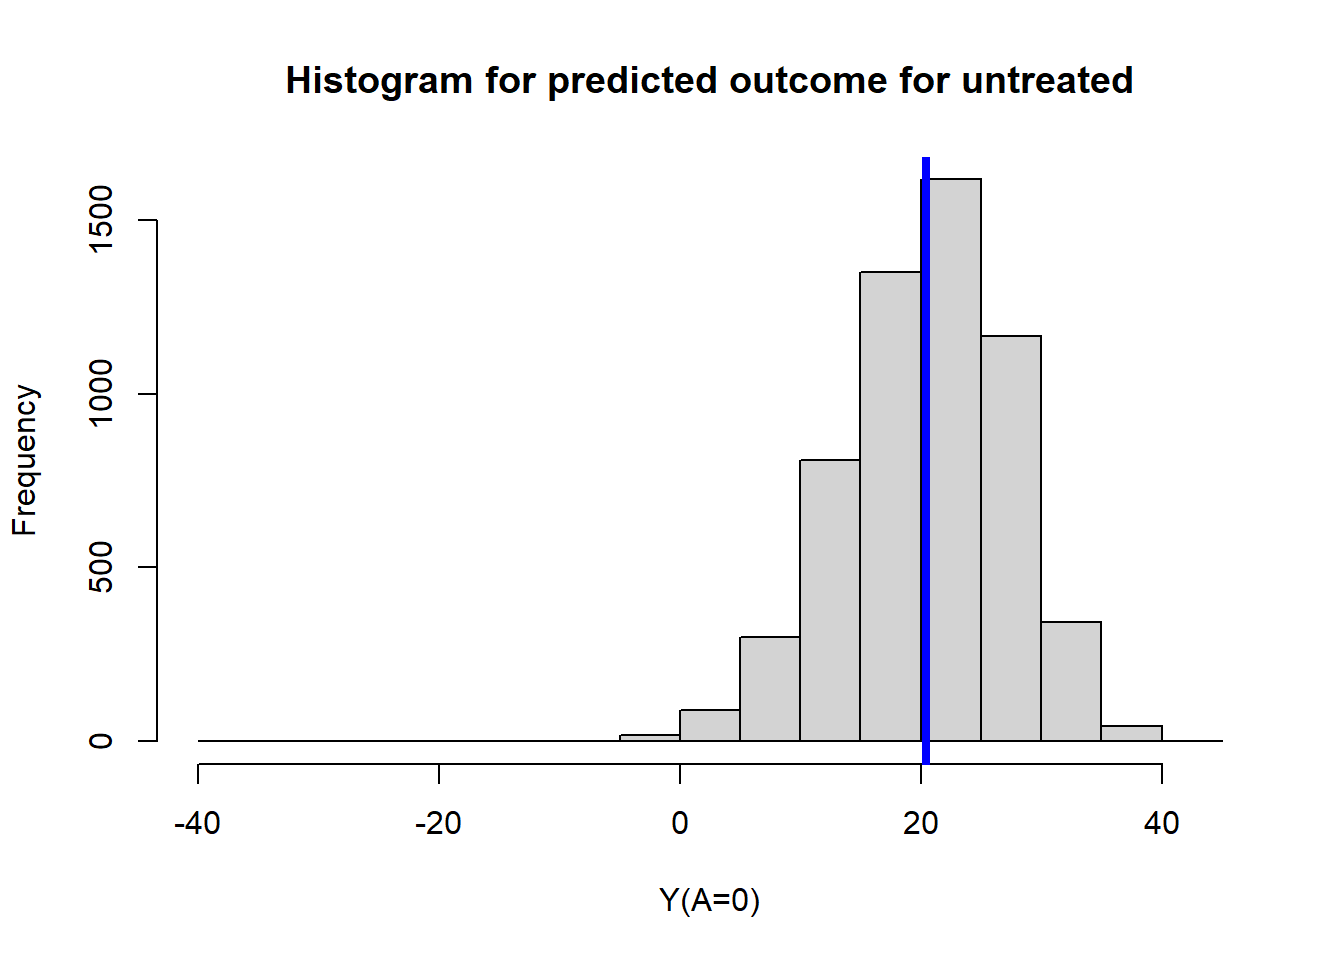
\includegraphics{TMLEw_files/figure-latex/reg2ac2-1.pdf}

\hypertarget{look-at-the-predicted-outcome-data-for-untreated}{%
\subsection{Look at the predicted outcome data for untreated}\label{look-at-the-predicted-outcome-data-for-untreated}}

\begin{Shaded}
\begin{Highlighting}[]
\NormalTok{small.data0 }\OtherTok{\textless{}{-}}\NormalTok{ ObsData[}\DecValTok{1}\SpecialCharTok{:}\DecValTok{6}\NormalTok{,}\FunctionTok{c}\NormalTok{(}\StringTok{"A"}\NormalTok{,}\StringTok{"Pred.Y0"}\NormalTok{)]}
\NormalTok{small.data0}\SpecialCharTok{$}\NormalTok{id }\OtherTok{\textless{}{-}} \FunctionTok{c}\NormalTok{(}\StringTok{"John"}\NormalTok{,}\StringTok{"Emma"}\NormalTok{,}\StringTok{"Isabella"}\NormalTok{,}\StringTok{"Sophia"}\NormalTok{,}\StringTok{"Luke"}\NormalTok{, }\StringTok{"Mia"}\NormalTok{)}
\NormalTok{small.data0 }\OtherTok{\textless{}{-}}\NormalTok{ small.data0[}\FunctionTok{c}\NormalTok{(}\StringTok{"id"}\NormalTok{, }\StringTok{"A"}\NormalTok{,}\StringTok{"Pred.Y0"}\NormalTok{)]}
\FunctionTok{kable}\NormalTok{(small.data0, }\AttributeTok{booktabs =} \ConstantTok{TRUE}\NormalTok{, }\AttributeTok{digits=}\DecValTok{1}\NormalTok{,}
             \AttributeTok{col.names =} \FunctionTok{c}\NormalTok{(}\StringTok{"id"}\NormalTok{,}\StringTok{"RHC status (A)"}\NormalTok{, }
                           \StringTok{"Y.hat when A=0 (no RHC)"}\NormalTok{))}
\end{Highlighting}
\end{Shaded}

\begin{tabular}{lrr}
\toprule
id & RHC status (A) & Y.hat when A=0 (no RHC)\\
\midrule
John & 0 & 14.6\\
Emma & 1 & 25.8\\
Isabella & 1 & 21.7\\
Sophia & 0 & 18.7\\
Luke & 1 & 10.7\\
\addlinespace
Mia & 0 & 22.6\\
\bottomrule
\end{tabular}

\hypertarget{look-at-the-predicted-outcome-data-for-all}{%
\subsection{Look at the predicted outcome data for all!}\label{look-at-the-predicted-outcome-data-for-all}}

\begin{Shaded}
\begin{Highlighting}[]
\NormalTok{small.data01 }\OtherTok{\textless{}{-}}\NormalTok{ small.data1}
\NormalTok{small.data01}\SpecialCharTok{$}\NormalTok{Pred.Y0 }\OtherTok{\textless{}{-}}\NormalTok{ small.data0}\SpecialCharTok{$}\NormalTok{Pred.Y0}
\NormalTok{small.data01}\SpecialCharTok{$}\NormalTok{Pred.TE }\OtherTok{\textless{}{-}}\NormalTok{ small.data01}\SpecialCharTok{$}\NormalTok{Pred.Y1 }\SpecialCharTok{{-}}\NormalTok{ small.data01}\SpecialCharTok{$}\NormalTok{Pred.Y0}
\NormalTok{m.Y1 }\OtherTok{\textless{}{-}} \FunctionTok{mean}\NormalTok{(small.data01}\SpecialCharTok{$}\NormalTok{Pred.Y1)}
\NormalTok{m.Y0 }\OtherTok{\textless{}{-}} \FunctionTok{mean}\NormalTok{(small.data01}\SpecialCharTok{$}\NormalTok{Pred.Y0)}
\NormalTok{mean.values }\OtherTok{\textless{}{-}} \FunctionTok{round}\NormalTok{(}\FunctionTok{c}\NormalTok{(}\ConstantTok{NA}\NormalTok{,}\ConstantTok{NA}\NormalTok{, m.Y1, m.Y0, m.Y1 }\SpecialCharTok{{-}}\NormalTok{m.Y0),}\DecValTok{1}\NormalTok{)}
\NormalTok{small.data2 }\OtherTok{\textless{}{-}} \FunctionTok{rbind}\NormalTok{(small.data01, mean.values)}
\FunctionTok{kable}\NormalTok{(small.data2, }\AttributeTok{booktabs =} \ConstantTok{TRUE}\NormalTok{, }\AttributeTok{digits=}\DecValTok{1}\NormalTok{,}
             \AttributeTok{col.names =} \FunctionTok{c}\NormalTok{(}\StringTok{"id"}\NormalTok{,}\StringTok{"RHC status (A)"}\NormalTok{,}
                           \StringTok{"Y.hat when A=1 (RHC)"}\NormalTok{,}
                           \StringTok{"Y.hat when A=0 (no RHC)"}\NormalTok{,}
                           \StringTok{"Treatment Effect"}\NormalTok{))}\SpecialCharTok{\%\textgreater{}\%}
  \FunctionTok{row\_spec}\NormalTok{(}\DecValTok{7}\NormalTok{, }\AttributeTok{bold =} \ConstantTok{TRUE}\NormalTok{, }\AttributeTok{color =} \StringTok{"white"}\NormalTok{, }\AttributeTok{background =} \StringTok{"\#D7261E"}\NormalTok{)}
\end{Highlighting}
\end{Shaded}

\begin{tabular}{lrrrr}
\toprule
id & RHC status (A) & Y.hat when A=1 (RHC) & Y.hat when A=0 (no RHC) & Treatment Effect\\
\midrule
John & 0 & 17.5 & 14.6 & 2.9\\
Emma & 1 & 28.7 & 25.8 & 2.9\\
Isabella & 1 & 24.6 & 21.7 & 2.9\\
Sophia & 0 & 21.6 & 18.7 & 2.9\\
Luke & 1 & 13.6 & 10.7 & 2.9\\
\addlinespace
Mia & 0 & 25.5 & 22.6 & 2.9\\
\cellcolor[HTML]{D7261E}{\textcolor{white}{\textbf{}}} & \cellcolor[HTML]{D7261E}{\textcolor{white}{\textbf{}}} & \cellcolor[HTML]{D7261E}{\textcolor{white}{\textbf{21.9}}} & \cellcolor[HTML]{D7261E}{\textcolor{white}{\textbf{19.0}}} & \cellcolor[HTML]{D7261E}{\textcolor{white}{\textbf{2.9}}}\\
\bottomrule
\end{tabular}

From this table, it is easy to calculate treatment effect estimate. The process we just went through, is a simplified version of \textbf{parametric G-computation}!

\hypertarget{parametric-g-computation}{%
\section{Parametric G-computation}\label{parametric-g-computation}}

\hypertarget{steps}{%
\subsection{Steps}\label{steps}}

\begin{enumerate}
\def\labelenumi{\arabic{enumi}.}
\tightlist
\item
  Fit the outcome regression on the exposure and covariates
\item
  Extract outcome prediction by setting all \(A=1\)
\item
  Extract outcome prediction by setting all \(A=0\)
\item
  Substract these two outcome predictions to get treatment effect estimate
\end{enumerate}

\begin{Shaded}
\begin{Highlighting}[]
\NormalTok{out.formula }\OtherTok{\textless{}{-}} \FunctionTok{as.formula}\NormalTok{(}\FunctionTok{paste}\NormalTok{(}\StringTok{"Y\textasciitilde{} A +"}\NormalTok{,}
                               \FunctionTok{paste}\NormalTok{(baselinevars,}
                                     \AttributeTok{collapse =} \StringTok{"+"}\NormalTok{)))}
\NormalTok{fit1 }\OtherTok{\textless{}{-}} \FunctionTok{lm}\NormalTok{(out.formula, }\AttributeTok{data =}\NormalTok{ ObsData)}
\NormalTok{ObsData}\SpecialCharTok{$}\NormalTok{Pred.Y1 }\OtherTok{\textless{}{-}} \FunctionTok{predict}\NormalTok{(fit1, }
                           \AttributeTok{newdata =} \FunctionTok{data.frame}\NormalTok{(}\AttributeTok{A =} \DecValTok{1}\NormalTok{, }
\NormalTok{                                                dplyr}\SpecialCharTok{::}\FunctionTok{select}\NormalTok{(ObsData, }\SpecialCharTok{!}\FunctionTok{c}\NormalTok{(A,Y))), }
                           \AttributeTok{type =} \StringTok{"response"}\NormalTok{)}
\NormalTok{ObsData}\SpecialCharTok{$}\NormalTok{Pred.Y0 }\OtherTok{\textless{}{-}} \FunctionTok{predict}\NormalTok{(fit1, }
                           \AttributeTok{newdata =} \FunctionTok{data.frame}\NormalTok{(}\AttributeTok{A =} \DecValTok{0}\NormalTok{, }
\NormalTok{                                                dplyr}\SpecialCharTok{::}\FunctionTok{select}\NormalTok{(ObsData, }\SpecialCharTok{!}\FunctionTok{c}\NormalTok{(A,Y))), }
                           \AttributeTok{type =} \StringTok{"response"}\NormalTok{)}
\NormalTok{ObsData}\SpecialCharTok{$}\NormalTok{Pred.TE }\OtherTok{\textless{}{-}}\NormalTok{ ObsData}\SpecialCharTok{$}\NormalTok{Pred.Y1 }\SpecialCharTok{{-}}\NormalTok{ ObsData}\SpecialCharTok{$}\NormalTok{Pred.Y0  }
\end{Highlighting}
\end{Shaded}

\hypertarget{treatment-effect-estimate}{%
\subsection{Treatment effect estimate}\label{treatment-effect-estimate}}

Mean value of predicted treatment effect

\begin{Shaded}
\begin{Highlighting}[]
\FunctionTok{mean}\NormalTok{(ObsData}\SpecialCharTok{$}\NormalTok{Pred.TE)}
\end{Highlighting}
\end{Shaded}

\begin{verbatim}
## [1] 2.90203
\end{verbatim}

SD of treatment effect

\begin{Shaded}
\begin{Highlighting}[]
\FunctionTok{sd}\NormalTok{(ObsData}\SpecialCharTok{$}\NormalTok{Pred.TE)}
\end{Highlighting}
\end{Shaded}

\begin{verbatim}
## [1] 5.132733e-15
\end{verbatim}

\begin{Shaded}
\begin{Highlighting}[]
\FunctionTok{hist}\NormalTok{(ObsData}\SpecialCharTok{$}\NormalTok{Pred.TE, }\AttributeTok{main =} \StringTok{"Histogram for predicted treatment effect"}\NormalTok{, }\AttributeTok{xlab =} \StringTok{"Y(A=1) {-} Y(A=0)"}\NormalTok{)}
\end{Highlighting}
\end{Shaded}

\begin{verbatim}
## Warning in plot.window(xlim, ylim, "", ...): relative range of values ( 93 *
## EPS) is small (axis 1)
\end{verbatim}

\begin{Shaded}
\begin{Highlighting}[]
\FunctionTok{abline}\NormalTok{(}\AttributeTok{v=}\FunctionTok{mean}\NormalTok{(ObsData}\SpecialCharTok{$}\NormalTok{Pred.TE),}\AttributeTok{col=}\StringTok{"blue"}\NormalTok{, }\AttributeTok{lwd =} \DecValTok{4}\NormalTok{)}
\end{Highlighting}
\end{Shaded}

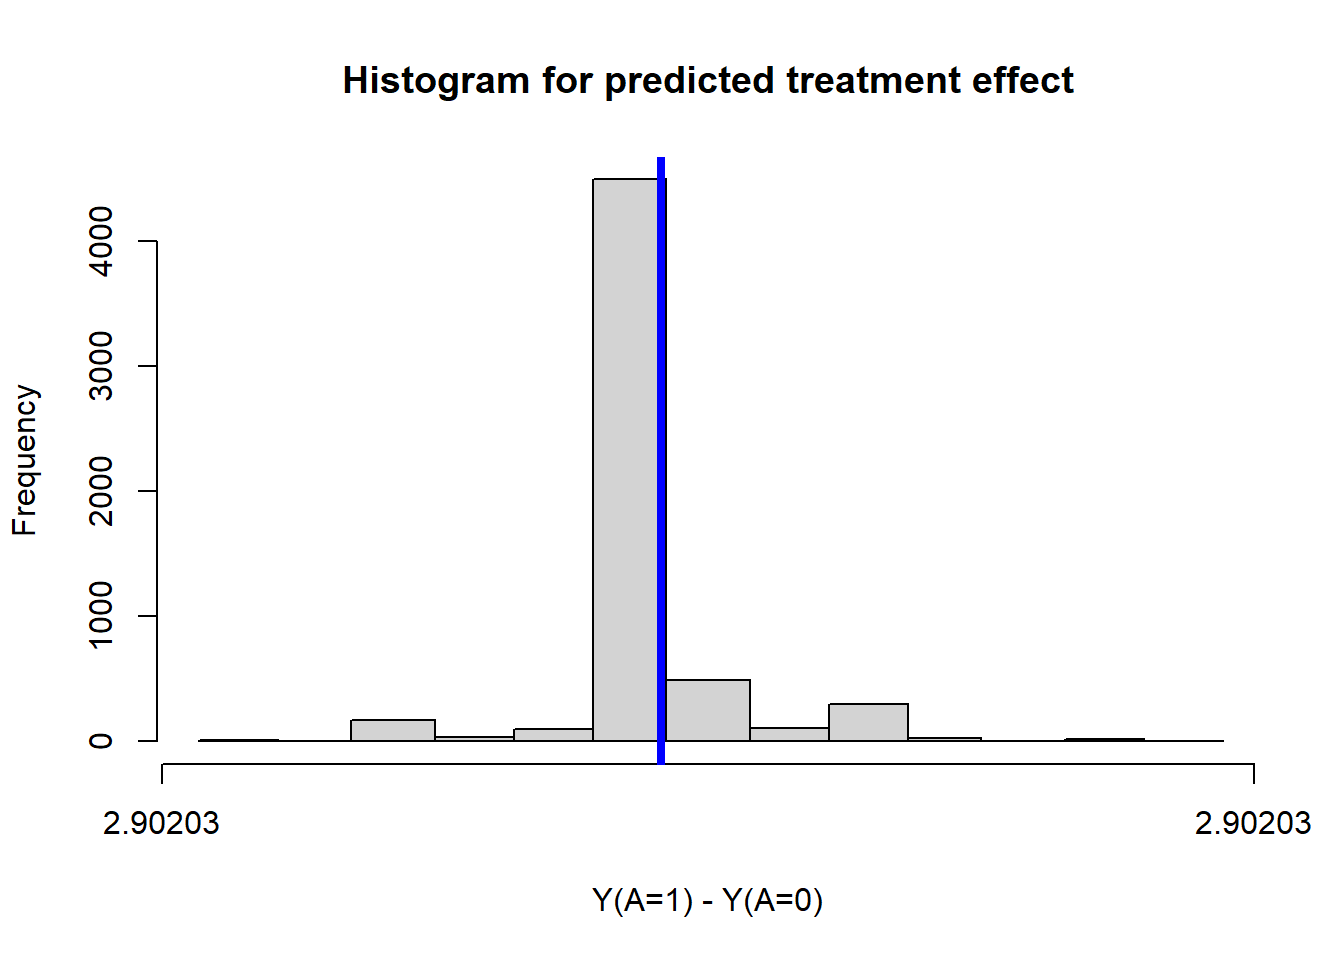
\includegraphics{TMLEw_files/figure-latex/reg2acnx3-1.pdf}

G-computation is highly sensitive to on model misspecification. Therefore, it is usually a good idea to use machine learning mehods that are flexible.

\hypertarget{g-computation-using-ml}{%
\section{G-computation using ML}\label{g-computation-using-ml}}

\hypertarget{a-tree-based-algorithm}{%
\subsection{A tree based algorithm}\label{a-tree-based-algorithm}}

XGBoost is a fast version of gradient boosting algotithm. Let us use this one to fit the data first.

\begin{Shaded}
\begin{Highlighting}[]
\FunctionTok{require}\NormalTok{(xgboost)}
\NormalTok{Y }\OtherTok{\textless{}{-}}\NormalTok{ObsData}\SpecialCharTok{$}\NormalTok{Y}
\NormalTok{ObsData.matrix }\OtherTok{\textless{}{-}} \FunctionTok{model.matrix}\NormalTok{(out.formula, }\AttributeTok{data =}\NormalTok{ ObsData)}
\NormalTok{fit3 }\OtherTok{\textless{}{-}} \FunctionTok{xgboost}\NormalTok{(}\AttributeTok{data =}\NormalTok{ ObsData.matrix, }
                \AttributeTok{label =}\NormalTok{ Y,}
                \AttributeTok{max.depth =} \DecValTok{10}\NormalTok{, }
                \AttributeTok{eta =} \DecValTok{1}\NormalTok{, }
                \AttributeTok{nthread =} \DecValTok{15}\NormalTok{, }
                \AttributeTok{nrounds =} \DecValTok{100}\NormalTok{, }
                \AttributeTok{alpha =} \FloatTok{0.5}\NormalTok{,}
                \AttributeTok{objective =} \StringTok{"reg:squarederror"}\NormalTok{, }
                \AttributeTok{verbose =} \DecValTok{0}\NormalTok{)}
\end{Highlighting}
\end{Shaded}

\hypertarget{extract-outcome-prediction-as-if-everyone-is-treated}{%
\subsection{Extract outcome prediction as if everyone is treated}\label{extract-outcome-prediction-as-if-everyone-is-treated}}

\begin{Shaded}
\begin{Highlighting}[]
\NormalTok{ObsData.matrix.A1 }\OtherTok{\textless{}{-}}\NormalTok{ ObsData.matrix }
\NormalTok{ObsData.matrix.A1[,}\StringTok{"A"}\NormalTok{] }\OtherTok{\textless{}{-}} \DecValTok{1}
\NormalTok{ObsData}\SpecialCharTok{$}\NormalTok{Pred.Y1 }\OtherTok{\textless{}{-}} \FunctionTok{predict}\NormalTok{(fit3, }\AttributeTok{newdata =}\NormalTok{ ObsData.matrix.A1)}
\FunctionTok{summary}\NormalTok{(ObsData}\SpecialCharTok{$}\NormalTok{Pred.Y1)}
\end{Highlighting}
\end{Shaded}

\begin{verbatim}
##    Min. 1st Qu.  Median    Mean 3rd Qu.    Max. 
## -24.061   7.997  15.990  23.417  29.978 393.987
\end{verbatim}

\hypertarget{extract-outcome-prediction-as-if-everyone-is-untreated}{%
\subsection{Extract outcome prediction as if everyone is untreated}\label{extract-outcome-prediction-as-if-everyone-is-untreated}}

\begin{Shaded}
\begin{Highlighting}[]
\NormalTok{ObsData.matrix.A0 }\OtherTok{\textless{}{-}}\NormalTok{ ObsData.matrix}
\NormalTok{ObsData.matrix.A0[,}\StringTok{"A"}\NormalTok{] }\OtherTok{\textless{}{-}} \DecValTok{0}
\NormalTok{ObsData}\SpecialCharTok{$}\NormalTok{Pred.Y0 }\OtherTok{\textless{}{-}} \FunctionTok{predict}\NormalTok{(fit3, }\AttributeTok{newdata =}\NormalTok{ ObsData.matrix.A0)}
\FunctionTok{summary}\NormalTok{(ObsData}\SpecialCharTok{$}\NormalTok{Pred.Y0)}
\end{Highlighting}
\end{Shaded}

\begin{verbatim}
##    Min. 1st Qu.  Median    Mean 3rd Qu.    Max. 
## -43.192   6.914  13.004  20.189  24.827 337.984
\end{verbatim}

\hypertarget{treatment-effect-estimate-1}{%
\subsection{Treatment effect estimate}\label{treatment-effect-estimate-1}}

\begin{Shaded}
\begin{Highlighting}[]
\NormalTok{ObsData}\SpecialCharTok{$}\NormalTok{Pred.TE }\OtherTok{\textless{}{-}}\NormalTok{ ObsData}\SpecialCharTok{$}\NormalTok{Pred.Y1 }\SpecialCharTok{{-}}\NormalTok{ ObsData}\SpecialCharTok{$}\NormalTok{Pred.Y0  }
\end{Highlighting}
\end{Shaded}

Mean value of predicted treatment effect

\begin{Shaded}
\begin{Highlighting}[]
\FunctionTok{summary}\NormalTok{(ObsData}\SpecialCharTok{$}\NormalTok{Pred.TE)}
\end{Highlighting}
\end{Shaded}

\begin{verbatim}
##      Min.   1st Qu.    Median      Mean   3rd Qu.      Max. 
## -195.6580   -0.9165    0.7056    3.2275    7.5578  177.9588
\end{verbatim}

\hypertarget{g-computation-using-superlearner}{%
\section{G-computation using SuperLearner}\label{g-computation-using-superlearner}}

\begin{Shaded}
\begin{Highlighting}[]
\FunctionTok{require}\NormalTok{(SuperLearner)}
\end{Highlighting}
\end{Shaded}

\hypertarget{superlearner-steps-by-available-package}{%
\subsection{SuperLearner Steps by available package}\label{superlearner-steps-by-available-package}}

\hypertarget{superlearner}{%
\subsubsection{SuperLearner}\label{superlearner}}

\hypertarget{treatment-effect-estimate-2}{%
\subsection{Treatment effect estimate}\label{treatment-effect-estimate-2}}

\hypertarget{iptw}{%
\chapter{IPTW}\label{iptw}}

\hypertarget{iptw-from-parametric-models}{%
\section{IPTW from parametric models}\label{iptw-from-parametric-models}}

\hypertarget{steps-1}{%
\subsection{Steps}\label{steps-1}}

\hypertarget{treatment-effect-estimate-3}{%
\subsection{Treatment effect estimate}\label{treatment-effect-estimate-3}}

\hypertarget{iptw-from-ml}{%
\section{IPTW from ML}\label{iptw-from-ml}}

\hypertarget{iptw-from-superlearner}{%
\section{IPTW from SuperLearner}\label{iptw-from-superlearner}}

\hypertarget{tmle}{%
\chapter{TMLE}\label{tmle}}

\hypertarget{transformation-of-continuous-outcome-variable}{%
\section{Transformation of continuous outcome variable}\label{transformation-of-continuous-outcome-variable}}

\hypertarget{initial-estimate}{%
\section{Initial estimate}\label{initial-estimate}}

\hypertarget{update}{%
\section{Update}\label{update}}

\hypertarget{treatment-effect-estimate-4}{%
\section{Treatment effect estimate}\label{treatment-effect-estimate-4}}

\hypertarget{pre-packaged-software}{%
\chapter{Pre-packaged software}\label{pre-packaged-software}}

\hypertarget{sl3}{%
\section{sl3}\label{sl3}}

\hypertarget{tmle-1}{%
\section{tmle}\label{tmle-1}}

\hypertarget{ltmle}{%
\section{ltmle}\label{ltmle}}

\hypertarget{tmle3}{%
\section{tmle3}\label{tmle3}}

\hypertarget{aipw}{%
\section{AIPW}\label{aipw}}

\hypertarget{rhc-results}{%
\section{RHC results}\label{rhc-results}}

\hypertarget{final-words}{%
\chapter{Final Words}\label{final-words}}

\hypertarget{why-sl-and-tmle}{%
\section{Why SL and TMLE}\label{why-sl-and-tmle}}

\hypertarget{prediction-goal}{%
\subsection{Prediction goal}\label{prediction-goal}}

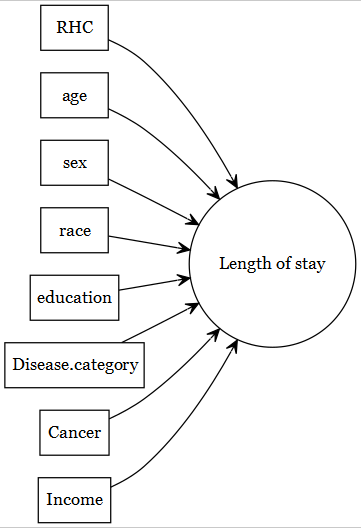
\includegraphics[width=5.01in]{images/dagpred}

\begin{itemize}
\tightlist
\item
  Assuming all covariates are measured, parametric models such as linear and logistic regressions are very efficient, but relies on strong assumptions. In real-world scenarios, it is often hard (if not impossible) to guess the correct specification of the right hand side of the regression equation.
\item
  Machine learning (ML) methods are very helpful for prediction goals. They are also helpful in identifying complex functions (non-linearities and non-additive terms) of the covariates (again, assuming they are measured).
\item
  There are many ML methods, but the procedures are very different, and they come with their own advantages and disadvantages. In a given real data, it is hard to apriori predict which is the best ML algorithm.
\item
  That's where super learner is helpful in combining strength from various algorithms, and producing 1 prediction column that has optimal statistical properties.
\end{itemize}

\hypertarget{causal-inference}{%
\subsection{Causal inference}\label{causal-inference}}

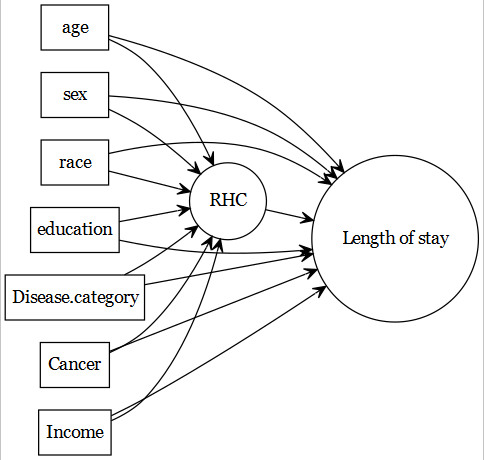
\includegraphics[width=6.72in]{images/dagci}

\begin{itemize}
\tightlist
\item
  For causal inference goals (when we have a primary exposure of interest), machine learning methods are often misleading. This is primarily due to the fact that they usually do not have an inherent mechanism of focusing on primary exposure (RHC in this example); and treats the primary exposure as any other predictors.
\item
  When using g-computation with ML methods, estimation of variance becomes a difficult problem. Generalized procedures such as robust SE or bootstrap methods are not supported by theory.
\item
  That's where TMLE methods shine, with the help of it's important statistical properties (double robustness, finite sample properties).
\end{itemize}

\hypertarget{identifiability-assumptions}{%
\subsection{Identifiability assumptions}\label{identifiability-assumptions}}

However, causal inference requires satisfying identifiability assumptions for us to interpret causality based on association measures from statistical models (see below). Many of these assumptions are not empirically testable. That is why, it is extremely important to work with \textbf{subject area experts} to assess the plausibility of those assumptions in the given context. No ML method, no matter how fancy it is, can automatically produce estimates that can be directly interpreted as causal, unless the identifiability assumptions are properly taken into account.

\begin{longtable}[]{@{}
  >{\raggedright\arraybackslash}p{(\columnwidth - 4\tabcolsep) * \real{0.33}}
  >{\raggedright\arraybackslash}p{(\columnwidth - 4\tabcolsep) * \real{0.33}}
  >{\raggedright\arraybackslash}p{(\columnwidth - 4\tabcolsep) * \real{0.33}}@{}}
\toprule
& & \\
\midrule
\endhead
Conditional Exchangeability & \(Y(1), Y(0) \perp A | L\) & Treatment assignment is independent of the potential outcome, given covariates \\
Positivity & \(0 < P(A=1 | L) < 1\) & Subjects are eligible to receive both treatment, given covariates \\
Consistency & \(Y = Y(a) \forall A=a\) & No multiple version of the treatment; and well defined treatment \\
\bottomrule
\end{longtable}

\hypertarget{further-reading}{%
\section{Further reading}\label{further-reading}}

\hypertarget{key-articles}{%
\subsection{Key articles}\label{key-articles}}

\begin{itemize}
\tightlist
\item
  TMLE Procedure:

  \begin{itemize}
  \tightlist
  \item
    \citet{luque2018targeted}
  \item
    \citet{schuler2017targeted}
  \end{itemize}
\item
  Super learner:

  \begin{itemize}
  \tightlist
  \item
    \citet{rose2013mortality}
  \item
    \citet{naimi2018stacked}
  \end{itemize}
\end{itemize}

\hypertarget{workshops}{%
\subsection{Workshops}\label{workshops}}

\begin{itemize}
\tightlist
\item
  \href{https://epiresearch.org/}{SER Workshop} Introduction to Parametric and Semi-parametric Estimators for Causal Inference by Laura B. Balzer \& Jennifer Ahern, 2020
\item
  \href{https://epiresearch.org/}{SER Workshop} Machine Learning and Artificial Intelligence for Causal Inference and Prediction: A Primer by Naimi A, 2021
\end{itemize}

\hypertarget{recorded-webinars}{%
\subsection{Recorded webinars}\label{recorded-webinars}}

The following webinars and workshops are freely accessible, and great for understanding the intuitions, theories and mechanisms behind these methods!

\begin{itemize}
\tightlist
\item
  \href{https://www.youtube.com/watch?v=PrPNP5RVcLg}{Targeted Machine Learning for Causal Inference based on Real World Data} by Mark van der Laan (Putnam Data Sciences)
\item
  \href{https://www.youtube.com/watch?v=8Q9dfW3oOi4}{An Introduction to Targeted Maximum Likelihood Estimation of Causal Effects} by Susan Gruber (Putnam Data Sciences)
\item
  \href{https://www.youtube.com/watch?v=1zT17HtvtF8}{An introduction to Super Learning} by Eric Polly (Putnam Data Sciences)
\item
  \href{https://www.youtube.com/watch?v=MDmddX267Ys}{Cross-validated Targeted Maximum Likelihood Estimation (CV-TMLE)} by Alan Hubbard (Putnam Data Sciences)
\item
  \href{https://www.youtube.com/watch?v=foY7HoCeo88}{Applications of Targeted Maximum Likelihood Estimation} by Laura Balzar (UCSF Epi \& Biostats)
\item
  \href{https://www.youtube.com/watch?v=2jumfnRQpxs}{Higher order Targeted Maximum Likelihood Estimation} by Mark van der Laan (Online Causal Inference Seminar)
\item
  \href{http://bcooltv.mcgill.ca/FDownloader.aspx?rid=e3143be2-918d-49d9-82ce-4dfea75ef1dc\&DLType=VGAMP4}{Targeted learning for the estimation of drug safety and effectiveness: Getting better answers by asking better questions} by Mireille Schnitzer (CNODES)
\item
  \href{https://www.cnodes.ca/online-lecture/targeted-learning-estimation/}{Applying targeted maximum likelihood estimation to pharmacoepidemiology} by Menglan Pang (CNODES)
\end{itemize}

\hypertarget{refs}{}
\begin{CSLReferences}{0}{0}
\end{CSLReferences}

  \bibliography{book.bib,packages.bib}

\end{document}
